\documentclass[a4paper,11pt]{article}
\setlength{\topmargin}{-.5in}
\setlength{\textheight}{9in}
\setlength{\oddsidemargin}{.125in}
\setlength{\textwidth}{6.25in}
\usepackage[pdftex]{graphicx}
\usepackage{fancyvrb}
\usepackage{hyperref}
\usepackage{float}

\makeatletter
\renewcommand\paragraph{%
   \@startsection{paragraph}{4}{0mm}%
      {-\baselineskip}%
      {.5\baselineskip}%
      {\normalfont\normalsize\bfseries}}
\makeatother

\begin{document}

% The Title page
\begin{titlepage}
\begin{center}

\includegraphics[width=0.6\textwidth]{fig/logo}\\[3cm]    
\textsc{\LARGE Patty / Mapping the Via Appia in 3D}\\[0.5cm]
\textsc{\large Via Appia 3D GIS: Software User Manual}\\[0.5cm]
\vfill
\end{center}
{\large
\emph{E. Ranguelova} \\
\emph{R. Goncalves } \\
\emph{R. van Haren } \\
\emph{O. Martinez-Rubi } \\
}
{\large
{Netherlands eScience Center, \\
Science Park 140 (Matrix 1), 1098 XG Amsterdam, the Netherlands\\
}
}
\begin{center}
{\large \today}
\end{center}
\end{titlepage}

\tableofcontents

\newpage
\section{Overview}
\label{sec:dataman_overview}

{\em begin remove after merging?} The subject of this project is an archaeological study of an area full of funerary monuments between the fifth and sixth miles of the Via Appia Antica. The data gathered from this area are of different resolution and different types (modalities): point clouds, meshes, photos, historical images and attribute information of the several monuments. The data are managed, processed and visualized by the Via Appia 3D GIS. The GIS combines a 3D viewer and a database (DB) and allows the user to refine which data are visualized based on some attributes. The system, which can be updated when new data is available, allows multiple researchers in different locations to analyze and study the area in 3D and aims to be an example for other complex archaeological study areas. {\em end remove after merging?} This document ({\em change to chapter after merging as part of the full Patty documentation?}) is the user manual for the data management part of the system.

The Via Appia 3D GIS has client-server architecture described in Section \ref{sec:}.

 The data are heterogeneous in nature both due to their conceptual difference and acquisition modality. The conceptual data description can be found in Section \ref{sec:concept_descr}. 

The storage of the data is organized according to a predefined hierarchical convention as described in Section \ref{sec:data_structure}. The database (DB) storing the actual data location as well as many attribute data (meta-data) of archaeological interest is explained in Section \ref{sec:}.   

\section{System architecture}

The developed 3D/4D GIS system has a two-tier architecture (Figure \ref{fig:sys_arch_2tier}). The {\em server} contains the master copy of the data and a PostgreSQL database called \textit{viaappiadb}. The {\em clients} download or request the data required for visualization and run the 3D/4D viewer locally or via a Web application which connects to the remote database when required.
 
A diagram of the data preparation framework which is executed in the server is shown in Figure \ref{fig:sys_arch_data_framework}. The raw data is converted to the OpenSceneGraph (http://www.openscenegraph.org) binary format. The \textit{viaappiadb} database is filled with meta-data information of the location of the raw data and the converted data. The archaeological information with attribute data for the several sites is provided in a Microsoft Access file. It needs to be converted to the PostgreSQL format before being imported into the main database. The footprints are provided in a PostgreSQL dump file and are imported into the \textit{viaappiadb} database as well.

\begin{figure}[!ht]
 \centering
 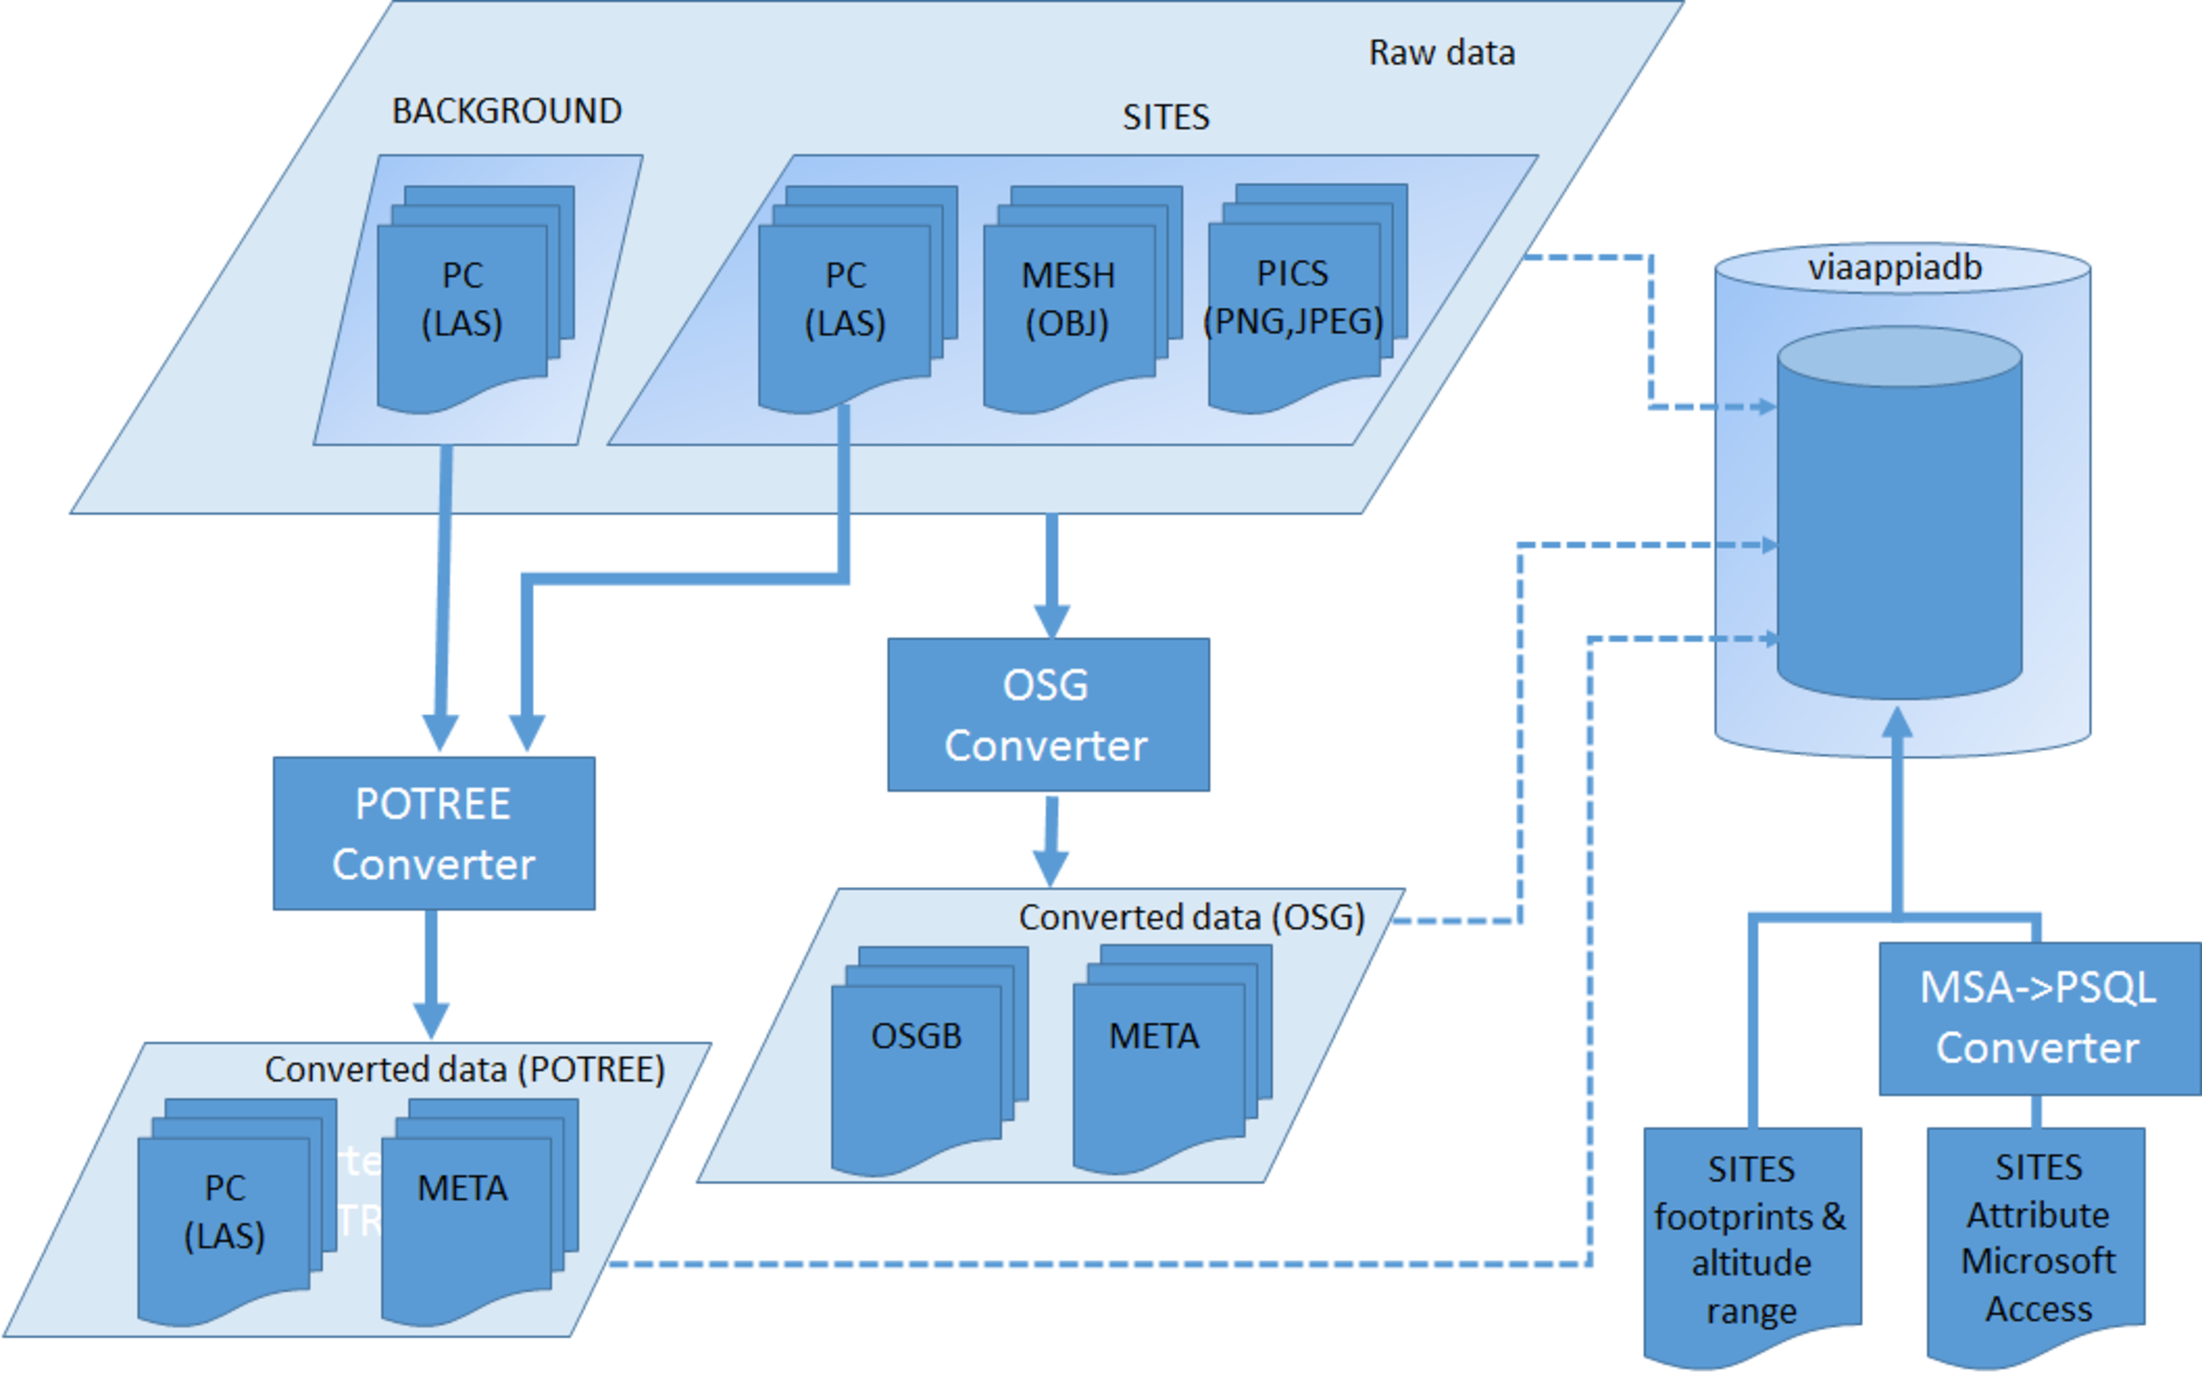
\includegraphics[width=0.4\textwidth]{fig/system_architecture/DataFramework.pdf}
 \caption{}
 \label{fig:sys_arch_data_framework}
\end{figure}

\begin{figure}[!ht]
 \centering
 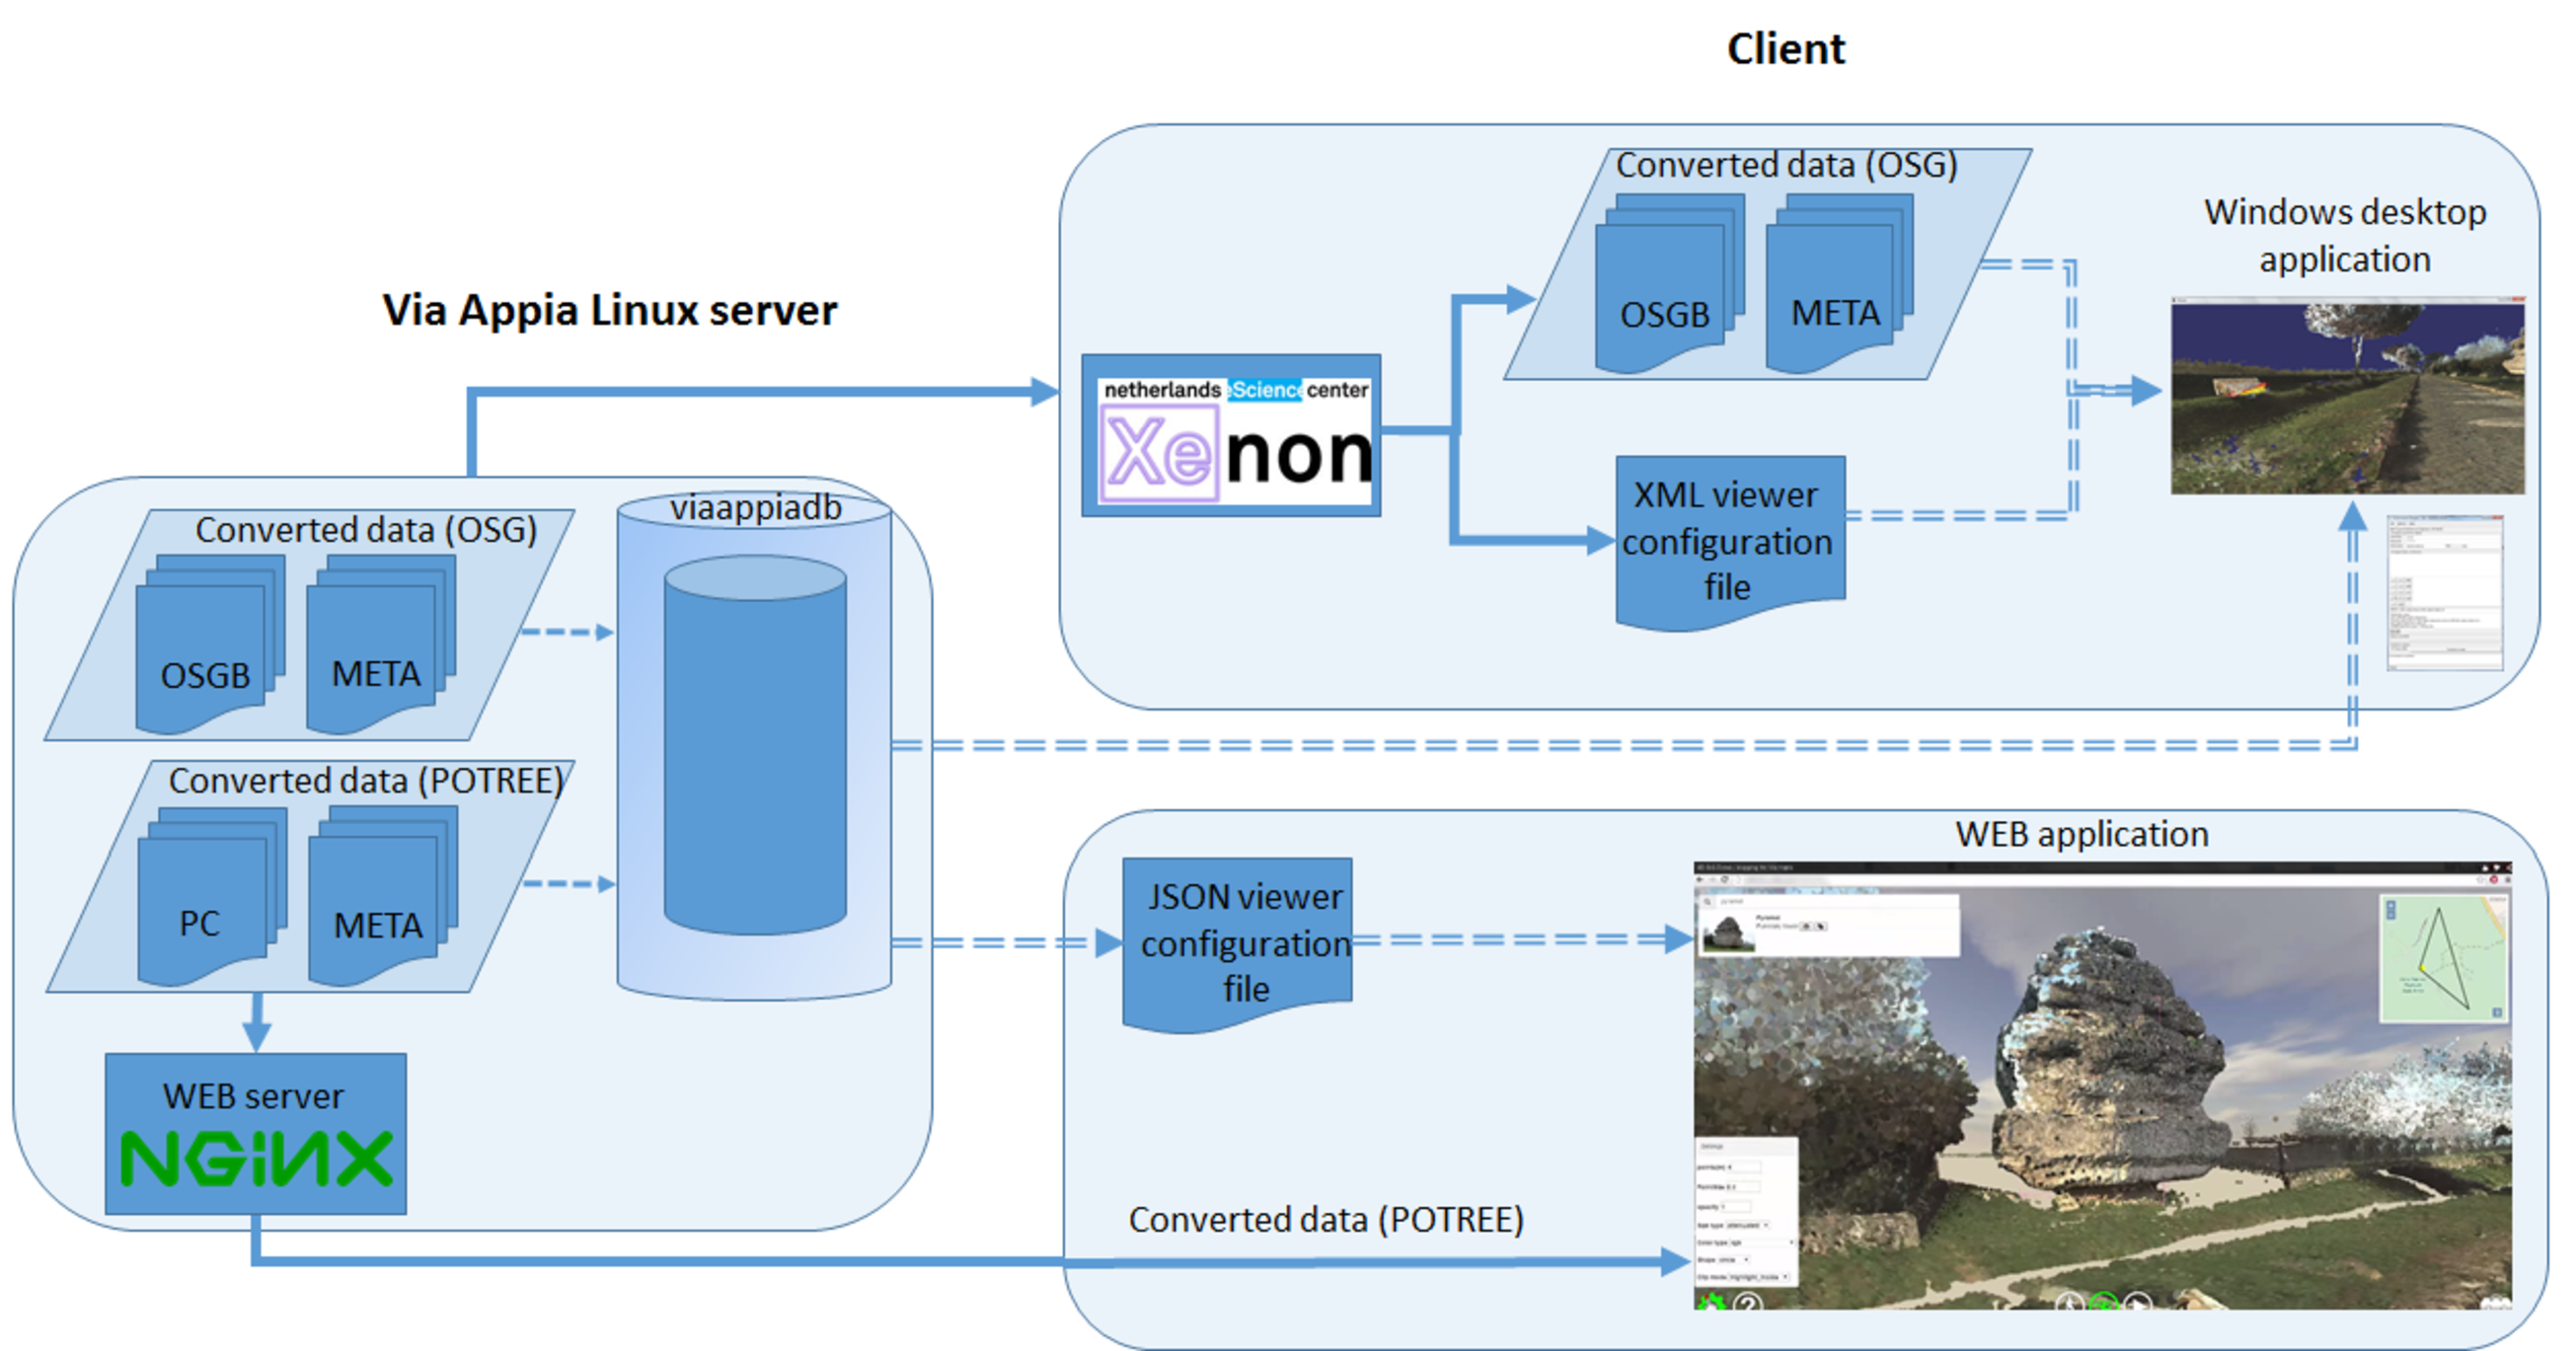
\includegraphics[width=0.4\textwidth]{fig/system_architecture/TwoTierArchitecture.pdf}
 \caption{}
 \label{fig:sys_arch_2tier}
\end{figure}

\section{Conceptual description}
\label{sec:concept_descr}

The gathered data of interest originate from the surface of an area corresponding to one mile of the ancient Via Appia in Rome. Conceptually these are divided into road data (also referred as to the {\em background}), which serve as a reference system and context and monument data, which represent the objects of interest, aligned with the road data. The monuments, are referred to as {\em sites}. 

The data, depending on the way of acquisition, are of several types:
\begin{itemize}
\item {\em Point clouds (PC)}
\begin{itemize}
\item A low resolution PC of the research area that has been generated making use of Fugro's DRIVE-MAP services. 
\item High resolution PCs of the different objects of interest (monuments, sites) generated using photogrammetric technologies. 
\end{itemize}
\item {\em Meshes} (sites reconstructions) for different historical epochs. 
\item Contemporary and historical {\em pictures} or paintings. 
\item {\em Attributes} data for the sites and their parts, which are gathered by field observations. 
\end{itemize}

\subsection{Point clouds}
Using the DRIVE-MAP service of Fugro the part of the surface of the Via Appia between the fifth and sixth miles was scanned and a {\em PC} was produced. A point in the PC has 3D coordinates ($x, y, z$), in respect to a given Earth reference system known at scanning time, color and possibly other measured attributes. The resolution (number of points per area or volume) of this point cloud is not enough to see detailed features of the sites, furthermore, they were only scanned from the main road. Thus, the back of the sites is missing. This is illustrated on Fig.\ref{fig:viaAppiaPointCloud}.

\begin{figure}[!ht]
\centering
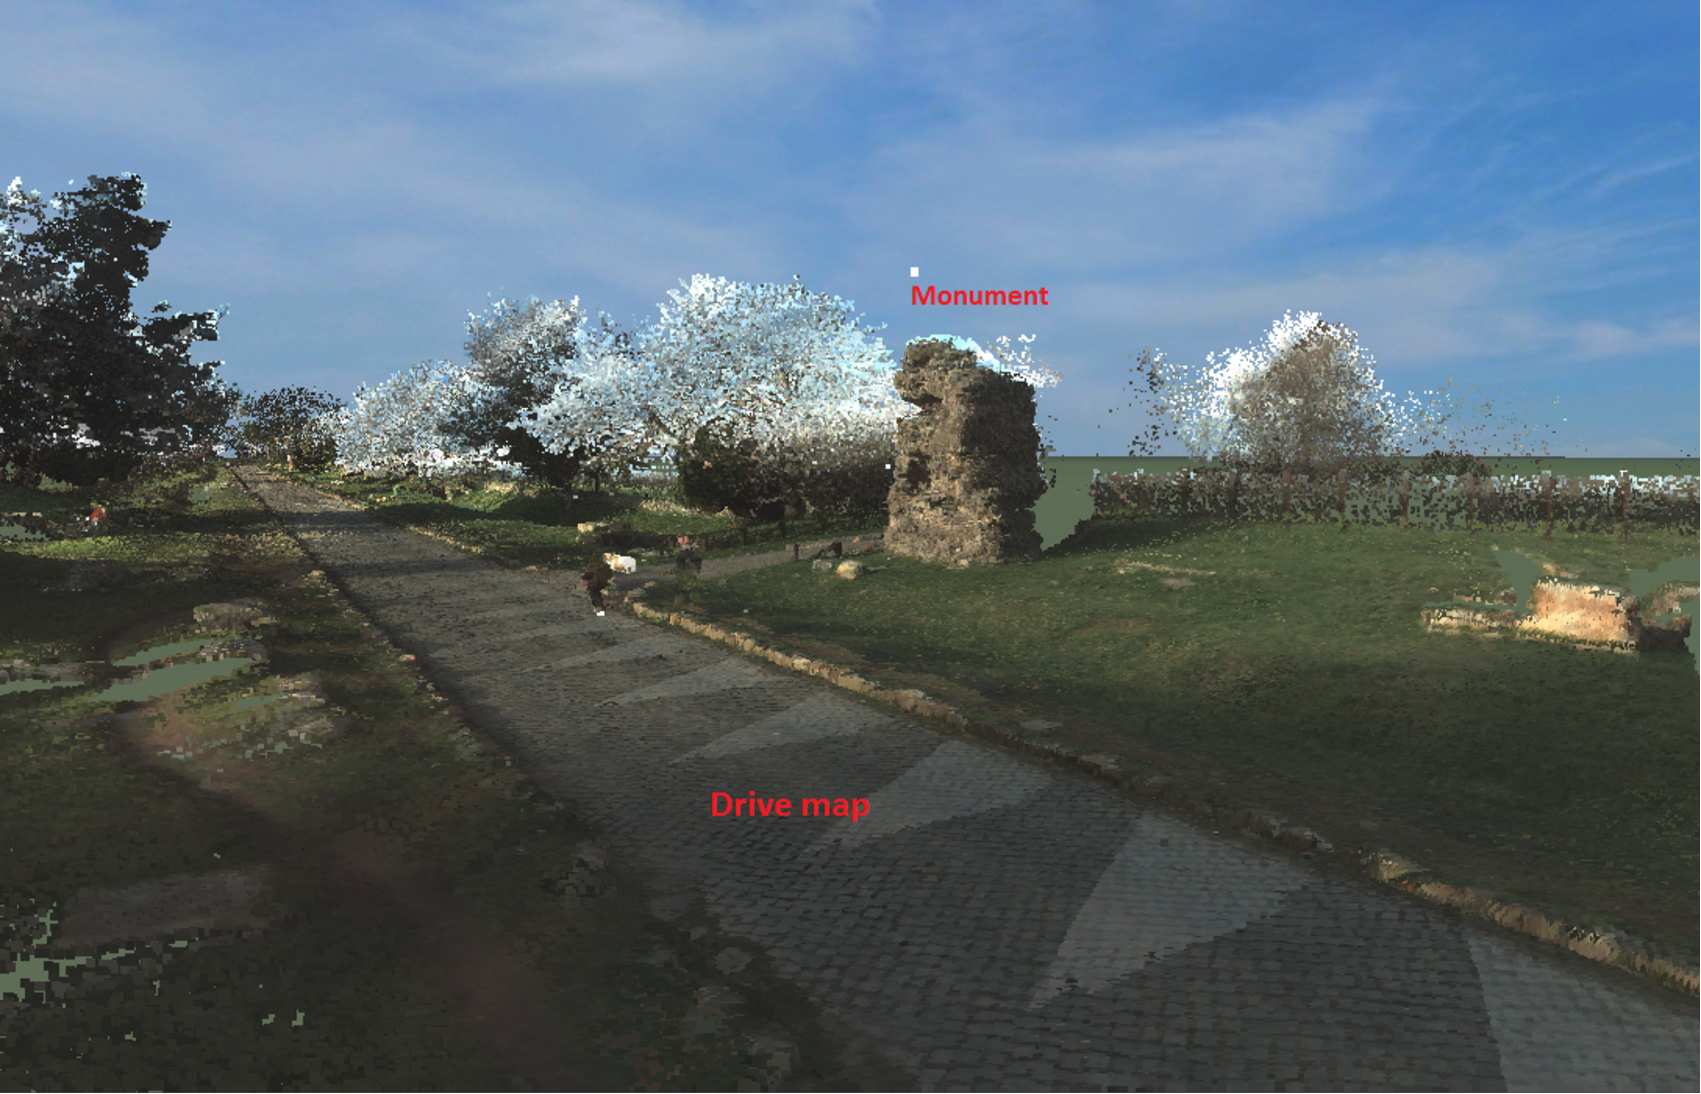
\includegraphics[scale=0.5]{fig/conceptual_description/ViaAppiaPCAnnot.pdf}
\caption{Point cloud data gathered along Via Appia. The Drive map is of low resolution and covers only part of the monuments (sites) facing the road.}
\label{fig:viaAppiaPointCloud}
\end{figure}

Usually there is one drive-map used as a background at a time, while there can be multiple drive-maps obtained at different times or acquisition devices. Or there can be different versions of the same drive-map where some post-processing have been performed like points classification (e.g.\ sky, tree, road, etc.) and possibly non-interesting points filtering (e.g.\ tree and grass removal).

Additional point clouds of higher resolution covering also the back of the monuments have been obtained using photogrammetric software from photographic pictures of the sites from different camera locations (viewpoints). 

\subsection{Pictures}
The pictures of a site can be both contemporary (current) or historical pictures or paintings. An illustration of visualizing a contemporary photo of a monument next to its point cloud data can be seen on Fig.\ref{fig:viaAppiaMeshPicture}. The photo was one of the photos used to generate the high resolution site PC and visualizing it next to the location of the monument can be extra informative or can be used as thumbnail. Usually there are multiple pictures per site.

\subsection{Meshes}
For the purpose of archaeological research, multiple reconstructions of the sites of interest are often performed. These reconstructions, or meshes, can also be current or historical. An illustration of visualizing a contemporary mesh of a monument aligned to its point cloud data can be seen on Fig.\ref{fig:viaAppiaMeshPicture}.

\begin{figure}[!ht]
\centering
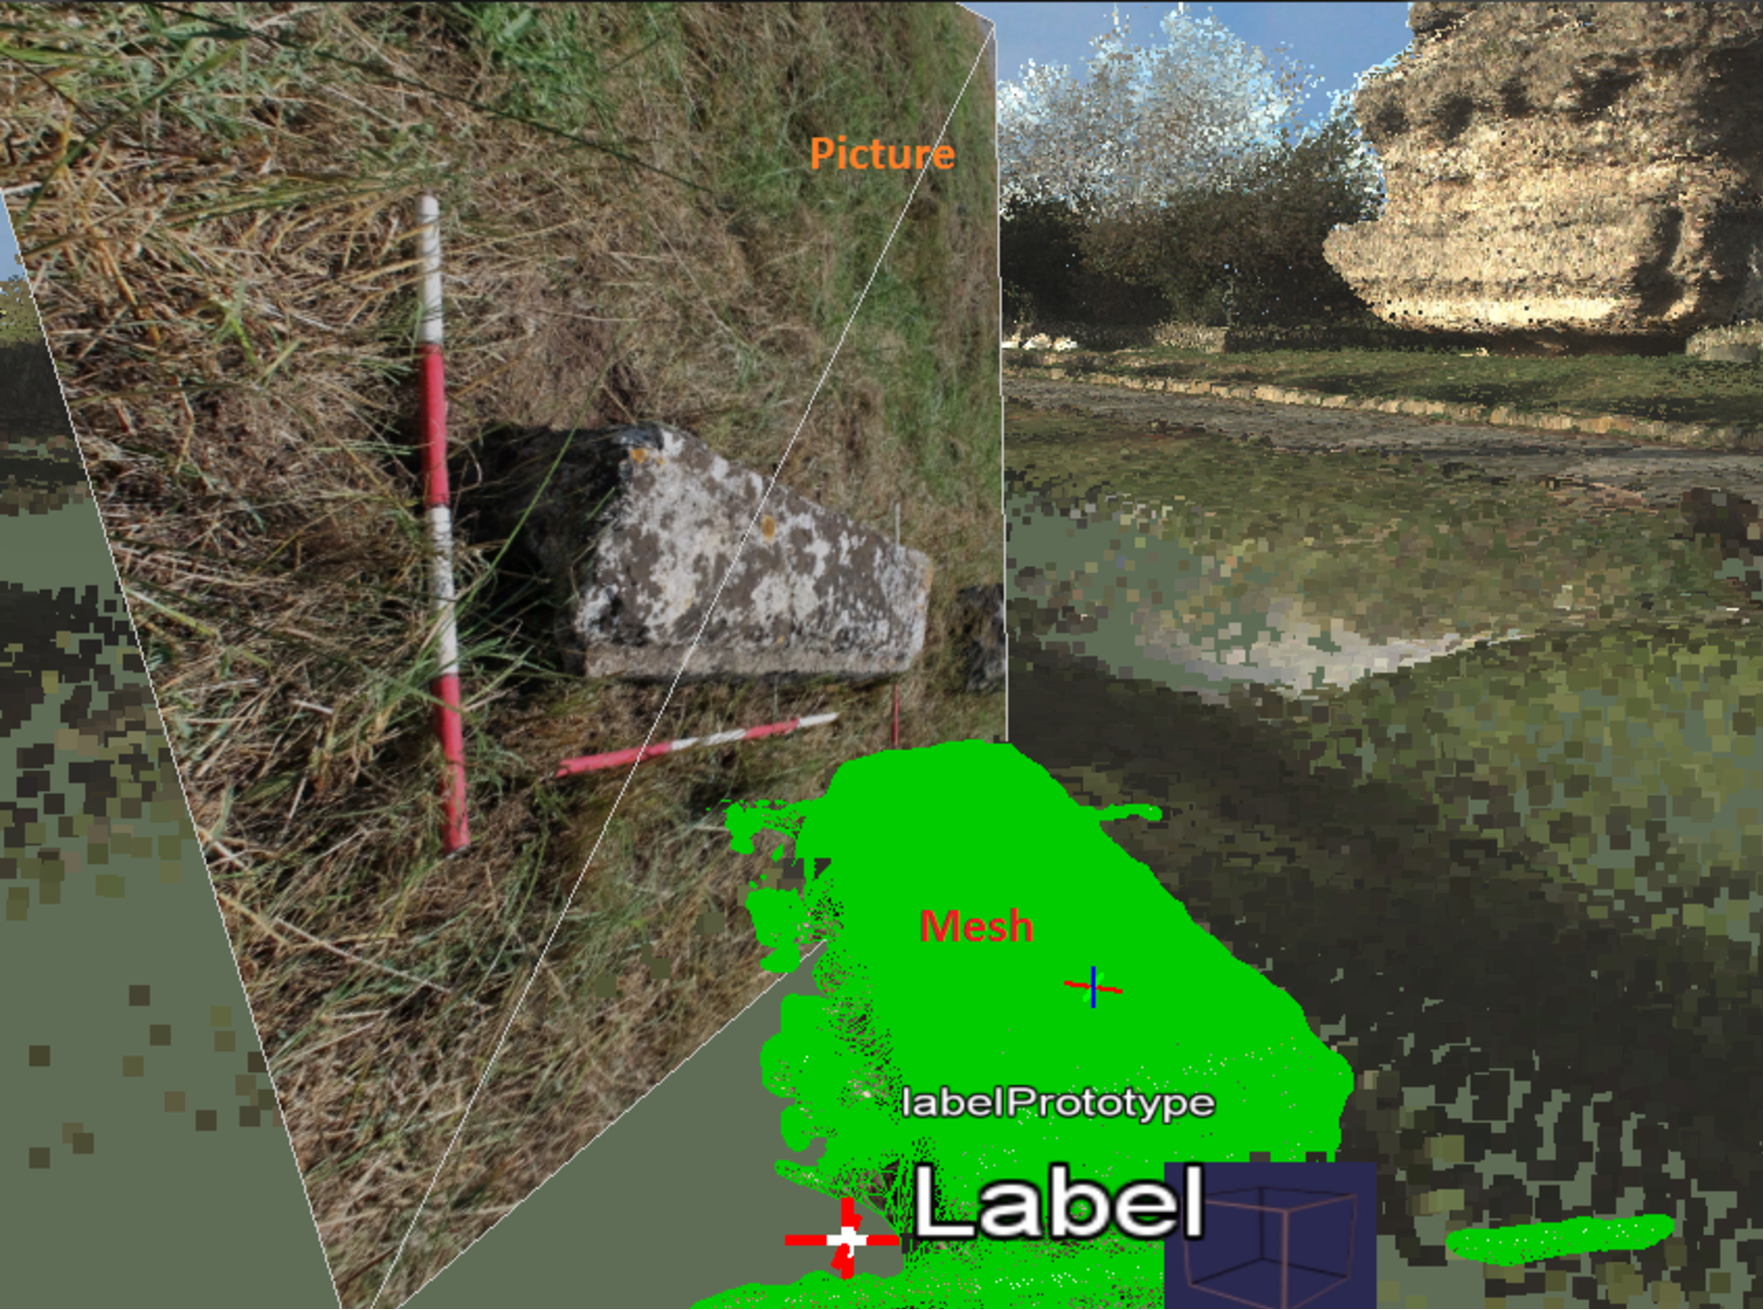
\includegraphics[scale=0.5]{fig/conceptual_description/ViaAppiaMeshPicture.pdf}
\caption{Reconstruction meshes and picture of a site overlayed on the point cloud data.}
\label{fig:viaAppiaMeshPicture}
\end{figure}


The point clouds, meshes and pictures are stored according to the data structure convention (Section \ref{sec:})

\subsection {Attributes}
These data are collected on the site from archaeologists. They are relevant to the archaeological research question,  and can be, for example material composition, condition, possible interpretation, description of the different elements or sub-parts, etc.  

The attribute data are considered as additional descriptive (meta) data and are stored in a database along with the pointers to the other data types (Section \ref{sec:}).

\section{Data structure}
\label{sec:data_structure}

\subsection{Description of the data structure}
\label{sec:descriptiondata}
The raw data is \textbf{only} stored in the Via Appia Linux server and there is Python script that needs to be used to generate the converted OSG data, the \textit{createosgdata.py}. The raw data directory is \textit{/home/vadata/DATA/RAW}. OSG data is stored in \textit{/home/vadata/DATA/OSG} and POTREE data is stored in \textit{/home/vadata/DATA/POTREE} (figure \ref{fig:directory_structure_overview}). 

The next subsections explores the RAW data tree in more detail and discusses how to modify and list the data in the RAW data tree.

\begin{figure}[!ht]
 \centering
 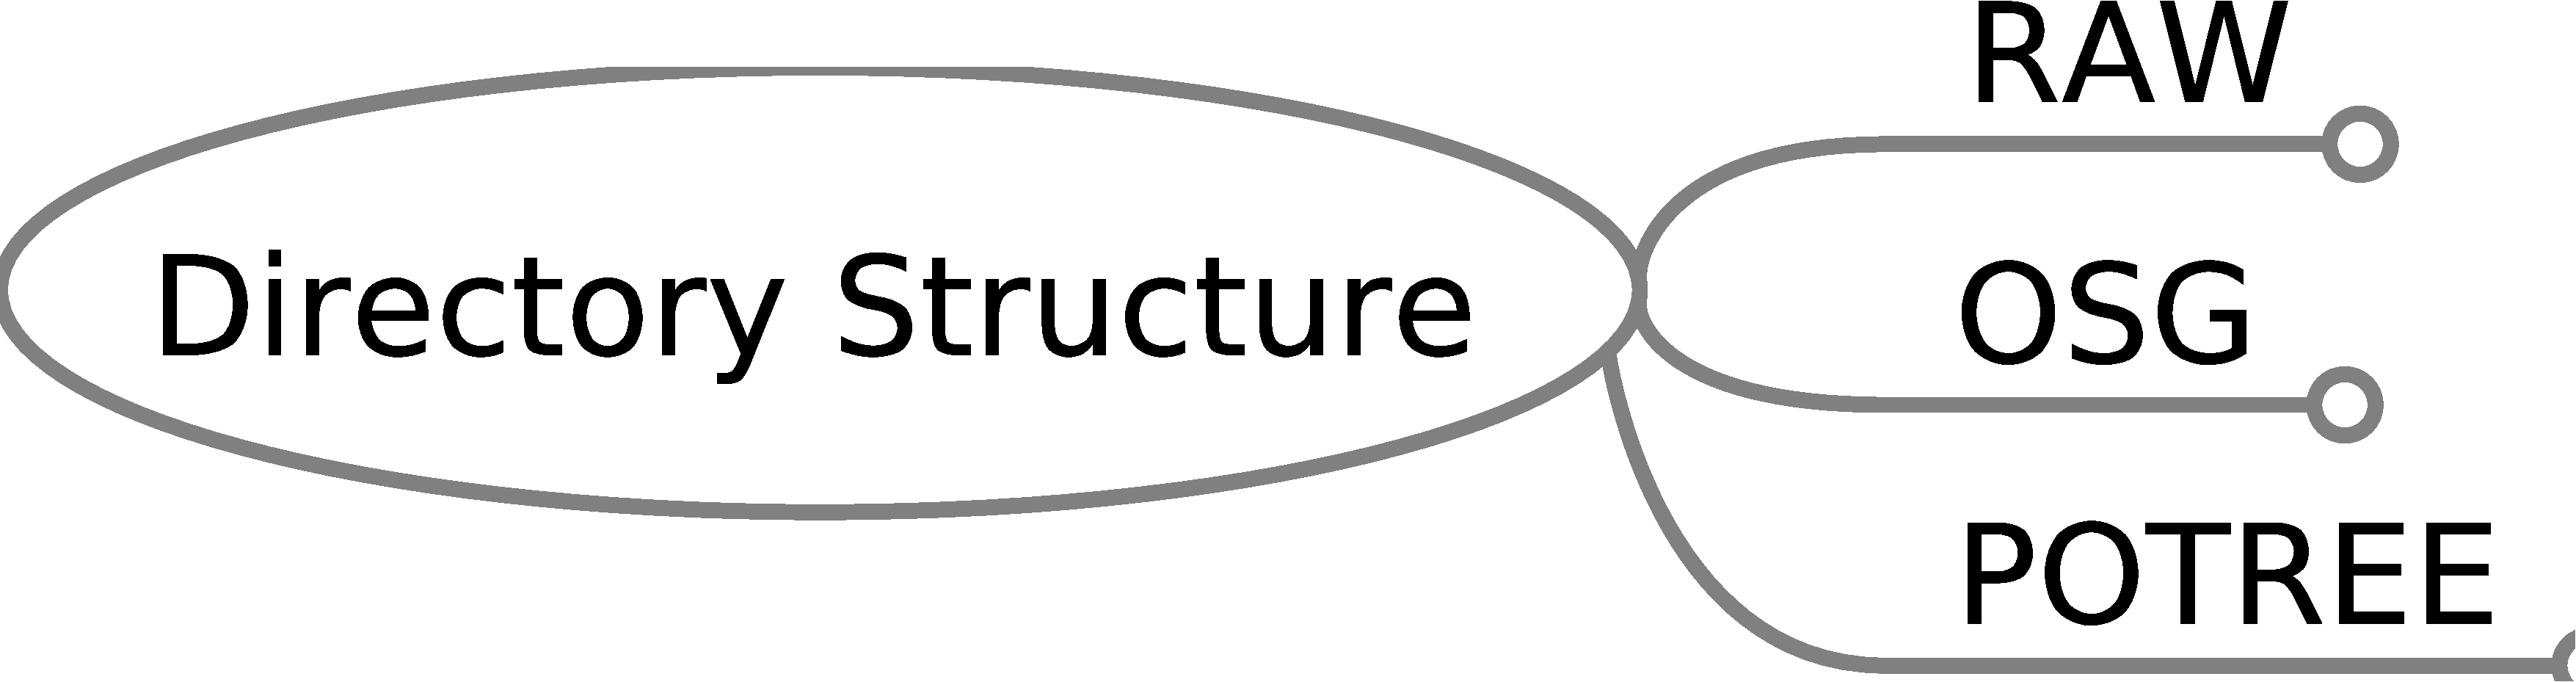
\includegraphics[width=0.4\textwidth]{fig/directory_structure_overview}
 \caption{Overview of the data structure}
 \label{fig:directory_structure_overview}
\end{figure}

\subsubsection{RAW data}
\paragraph{Point clouds}
Higher resolution point clouds are stored in the subdirectories \textit{PC/BACK} and \textit{PC/SITE}, for respectively backgrounds and sites. For backgrounds, the subdirectory contains different folders with point clouds for each background. For sites, the subdirectory contains a separate folder for each site (e.g.\ \textit{PC/SITE/S162} for site 162), which in turn contain different folders for each point cloud of the site. These folders contain LAS files of different point clouds of the site. 

The LAS files contained in each site subfolder may have been pre-aligned (using CloudCompare for example). In that case the LAS file name must be \textbf{*\_ALIGNED\_\textit{BGNAME}*} where \textit{BGNAME} must be the background name (as contained in the folder \textit{PC/BACK/}).
Some point clouds generation tools store the color information in 8 bits instead of the usual 16 bits. In that case the folder name must be \textbf{*\_8BC}. The effect of having an undeclared LAS file with 8 bit color is that the converted data will be black and white. Note that these properties are cumulative, for example \textit{S162\_ALIGNED\_DRIVE\_1\_V3\_8BC} is a valid name for a folder containing a LAS file with 8 bit color information and aligned points.

\begin{figure}[]
 \centering
 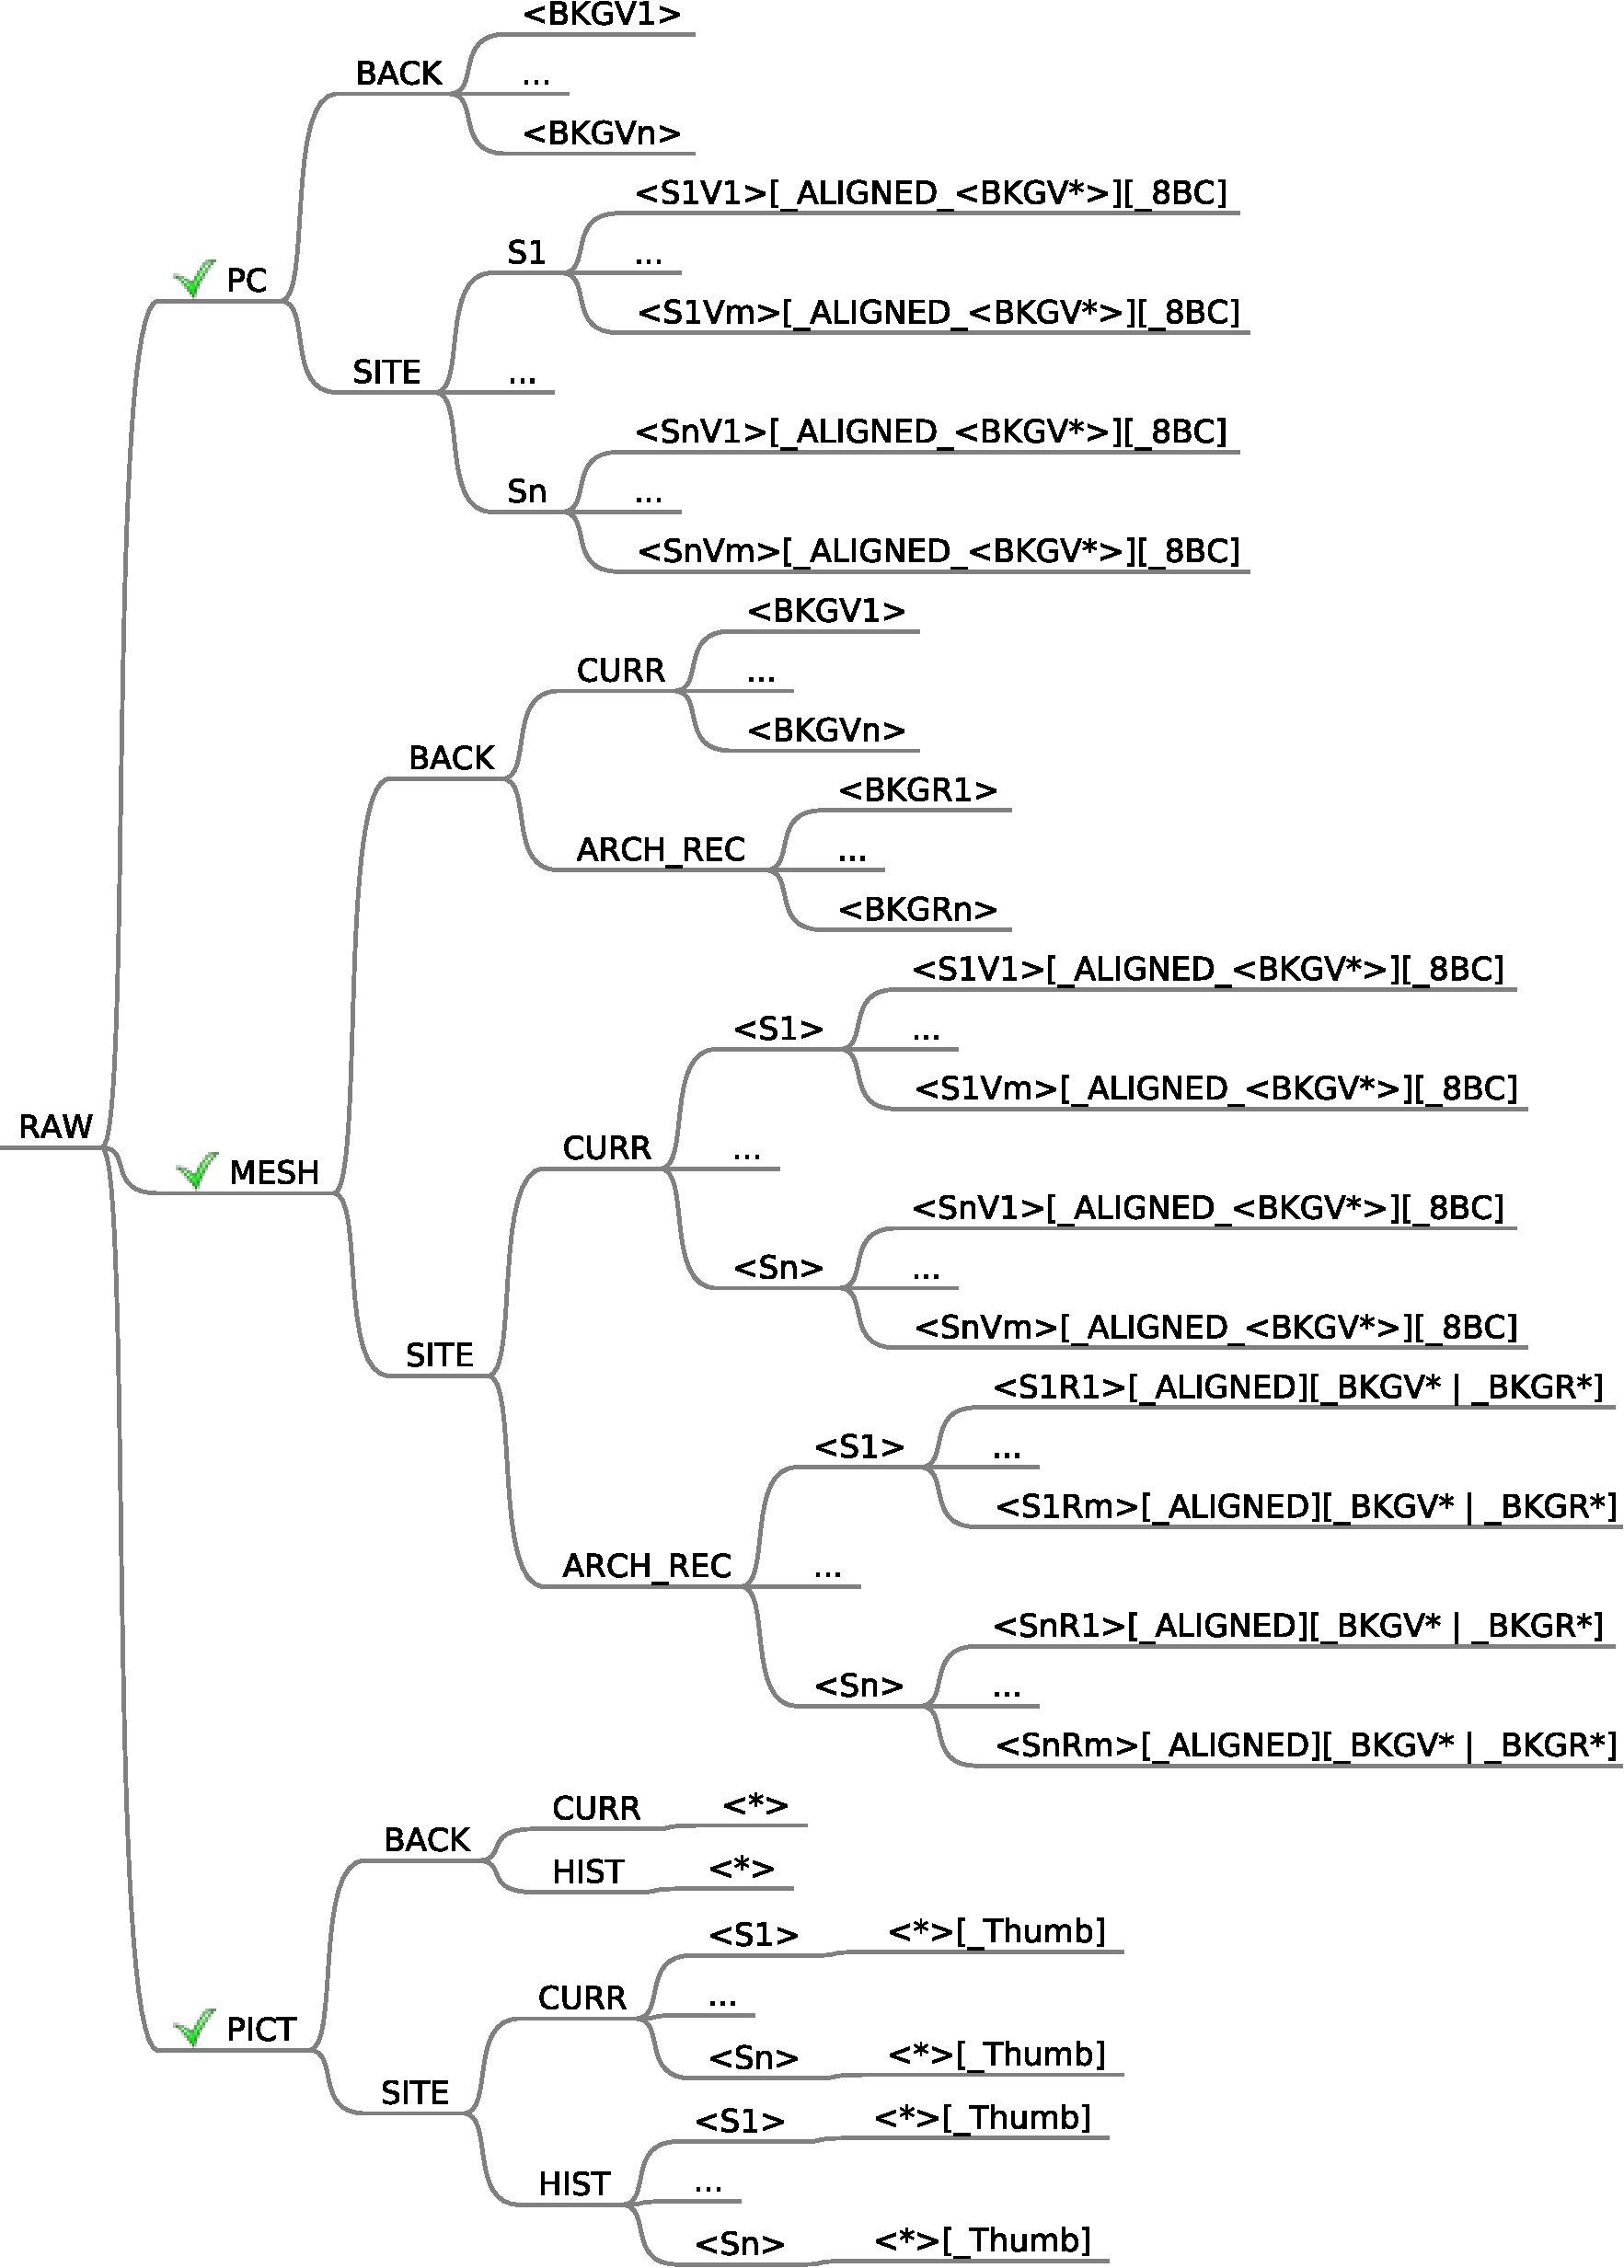
\includegraphics[width=0.8\textwidth]{fig/directory_structure_raw}
 \caption{Overview of the data structure: RAW data items}
 \label{fig:directory_structure_overview_raw}
\end{figure}


\paragraph{Meshes}
Meshes are stored in the directories \textit{MESH/BACK} and \textit{MESH/SITE}, for respectively backgrounds and sites. There are two types of meshes: (a) current  mesh representations, and (b) archeological reconstructions. For backgrounds, they are stored in respectively \textit{MESH/BACK/CURR} and \textit{MESH/BACK/ARCH\_REC}. For sites they are stored in respectively \textit{MESH/SITE/CURR} and \textit{MESH/SITE/ARCH\_REC}. For sites, each of these directories contain different folders for each site. For example the folder \textit{MESH/SITE/CURR/S162} contains mesh representations of the current state of the site 162. 

For each site there must be different folders for the several meshes. Inside these folders the files for the meshes are stored (OBJ, MTL, JPEG). For example \textit{MESH/SITE/CURR/S162} could contain two folders called \textit{162\_curr\_1} and \textit{162\_curr\_2} and each of them contain a OBJ, a MTL and several JPEG files. 

Similarly to the LAS files the meshes can also be aligned. In this case the folder name for a certain mesh must be \textbf{*\_ALIGNED\_\textit{BGNAME}*}. 

\paragraph{Pictures}
Pictures are stored in the subdirectory \textit{PICT}. Pictures can be either of a background or of a site. For both types a further subdivision is made between (a) pictures of the current state of the sites, and (b) historical pictures and paintings. These are stored in respectively \textit{PICT/BACK/CURR} and \textit{PICT/BACK/HIST} for backgrounds, or \textit{PICT/SITE/CURR} and \textit{PICT/SITE/HIST} for sites. For sites, each of these directoryes contains a separate folder for each site. For example the folder \textit{PICT/SITE/CURR/S162} contains pictures of the current state of the site 162.

\subsubsection{OSG data}
The raw data can be converted to the OSGB format. For that purpose a python script \textit{GenerateOSG.py} as been created (section \ref{sec:generatePOTree}). This script should be run with the \textit{vadata} user and should be run when some data has changed in the raw data directory. The POTree data is copied automatically in the POTree data tree, with the naming as specified in figure \ref{fig:directory_structure_overview_osg}.

In order to view the data in your Windows machine you need to download a version of the converted OSG data in your local machine. We use a NLeSC tool called Xenon.

\begin{figure}[!ht]
 \centering
 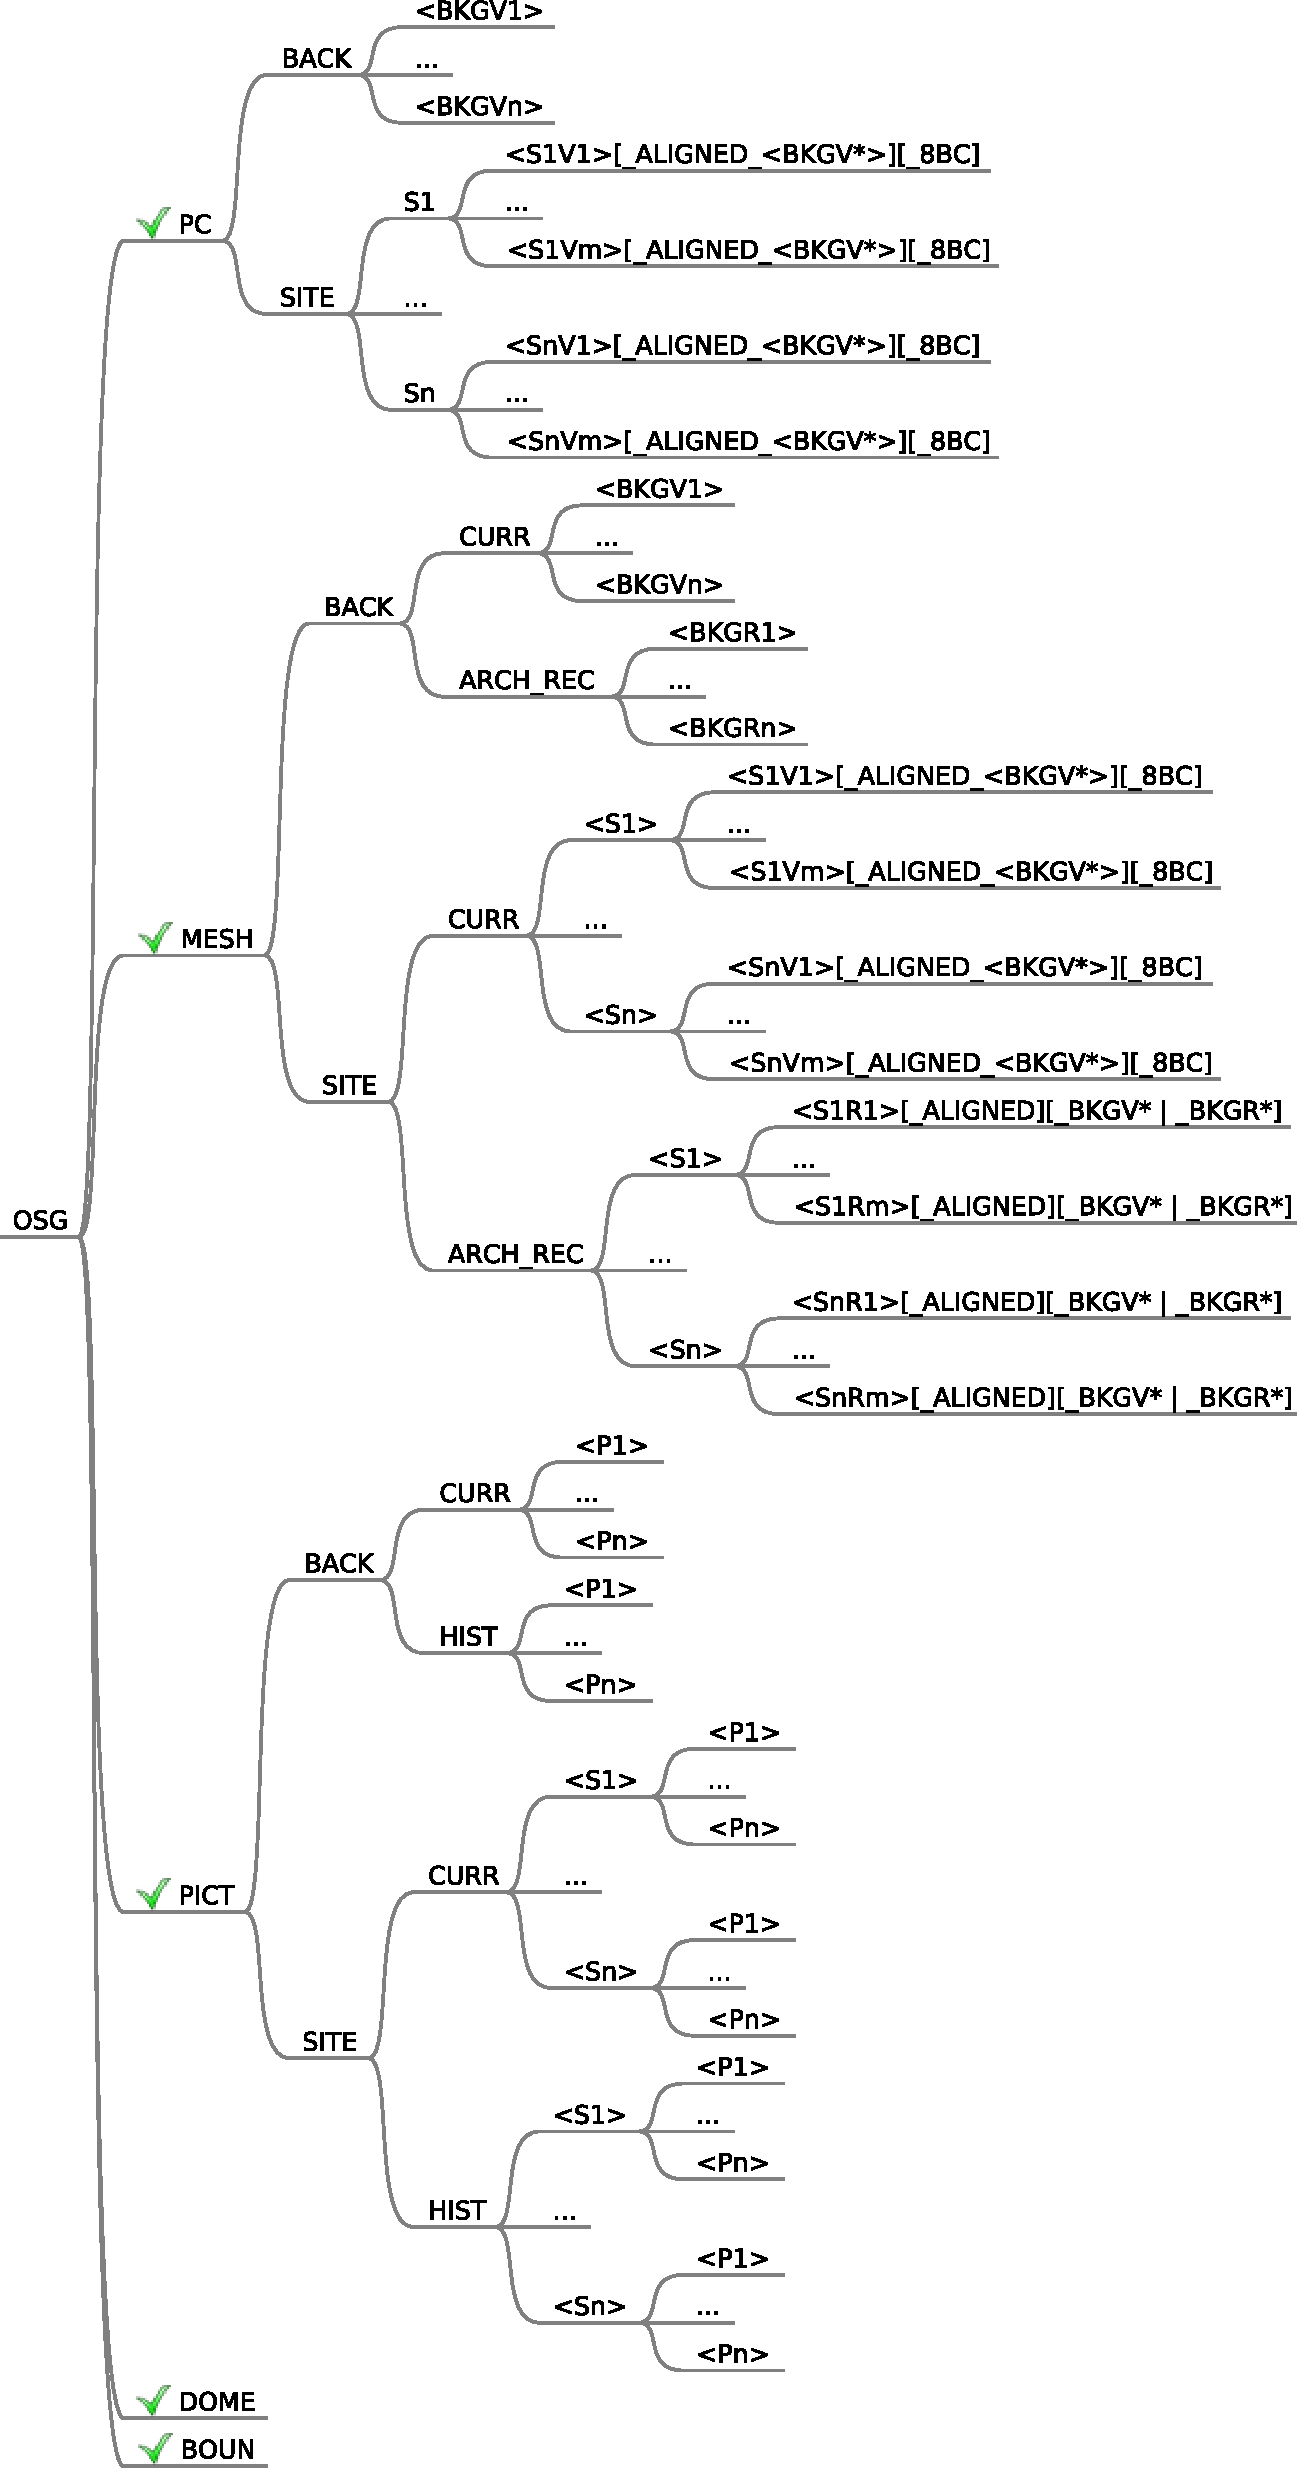
\includegraphics[width=0.75\textwidth]{fig/directory_structure_osg}
 \caption{Overview of the data structure: OSG data items}
 \label{fig:directory_structure_overview_osg}
\end{figure}

\subsubsection{POTree data}
The raw data can be converted to the POTree format. For that purpose a python script \textit{GeneratePOTree.py} has been created (section \ref{sec:generateosg}). This script should be run with the \textit{vadata} user and should be run when some data has changed in the raw data directory. The POTree data is copied automatically in the POTree data tree, with the naming as specified in figure \ref{fig:directory_structure_overview_potree}.

\begin{figure}[!ht]
 \centering
 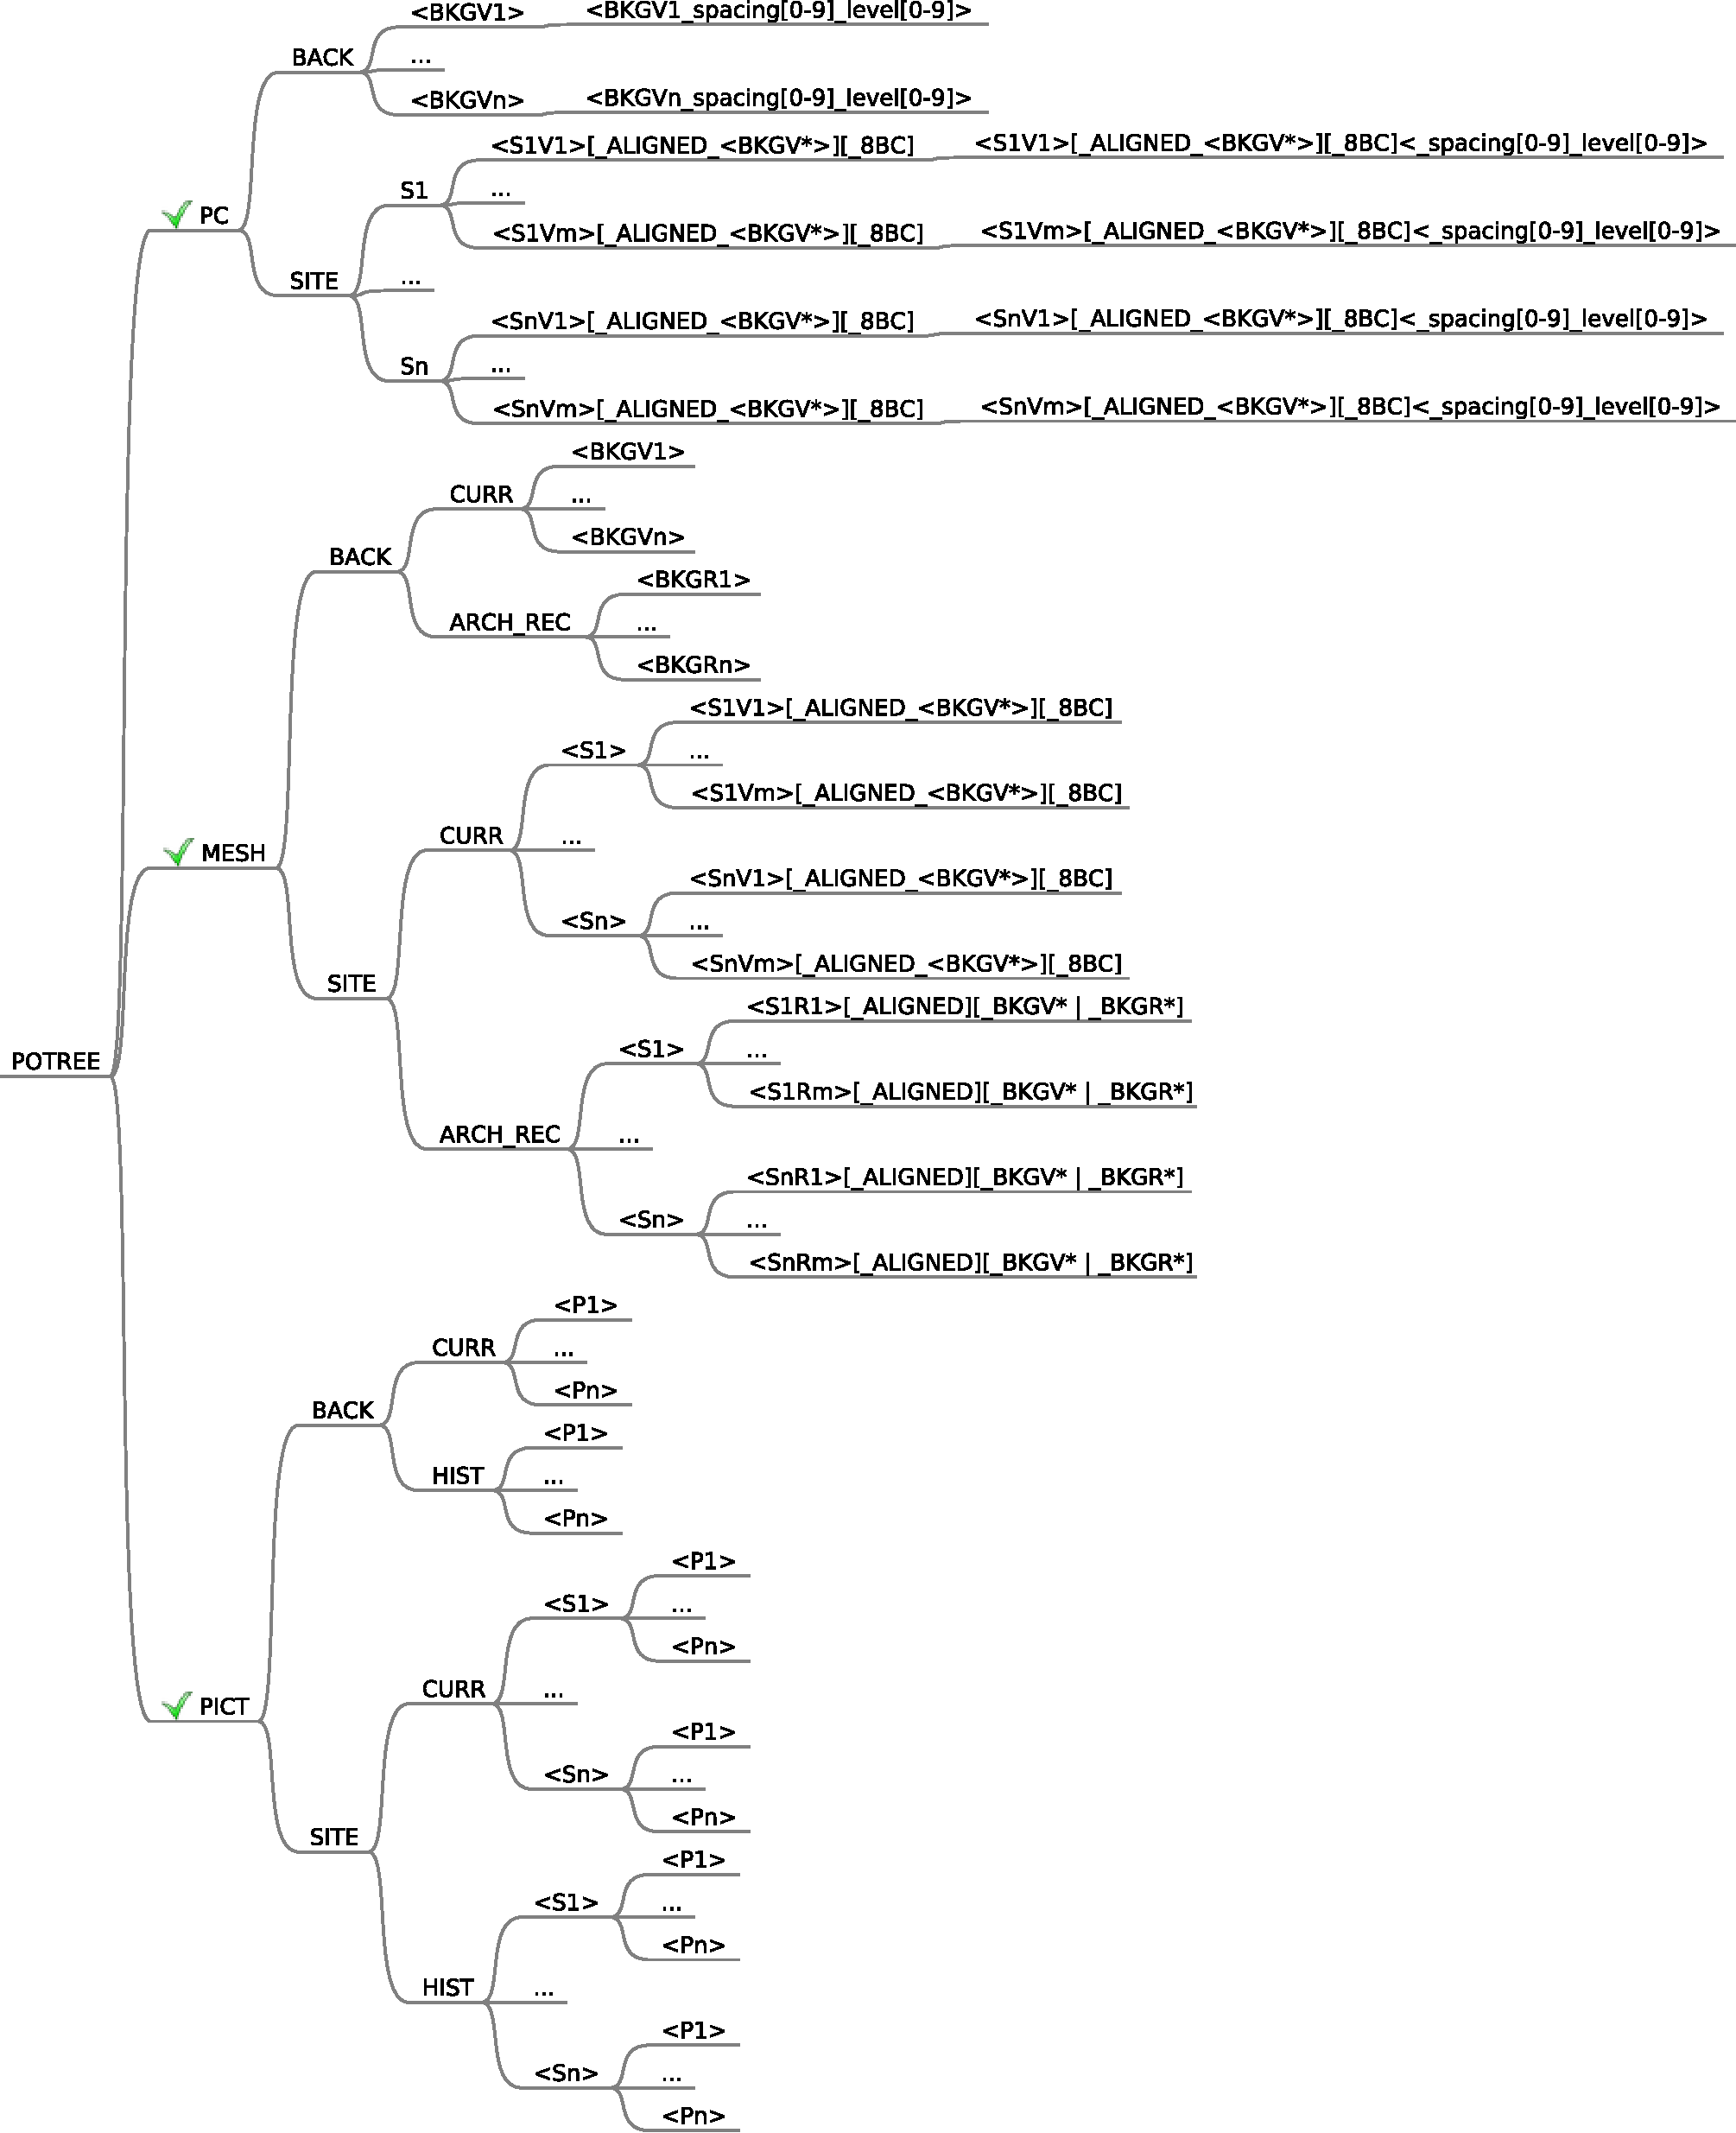
\includegraphics[width=1\textwidth]{fig/directory_structure_potree}
 \caption{Overview of the data structure: POTree data items}
 \label{fig:directory_structure_overview_potree}
\end{figure}


\subsection{Operation on the data structure}
Different operations can be performed on the data structure. The different operations that can be performed are (1) adding RAW data items (section \ref{sec:addraw}); (2) removing RAW data items (section \ref{sec:removeraw}); and (3) listing RAW data items (section \ref{sec:listraw}).

\subsubsection{Adding RAW data items}
\label{sec:addraw}
This section describes the script that should be used to add raw data items to the directory structure: \textit{AddRawDataItem.py}. To run the script, the user needs, depending on the exact datatype, supply additional arguments to the script. An overview of the possible arguments are found in the verbatim below. The script automatically creates a destination folder with the required naming, as specified in section \ref{sec:descriptiondata}, using the supplied arguments.

\begin{Verbatim}[fontfamily=courier,commandchars=\\\{\},fontsize=\footnotesize]
 usage: AddRawDataItem.py [-h] [-i DATA] -k {BACK,SITE} -t {PC,MESH,PICT} -f FILE                                                                                                     
             [-p {CURR,HIST,ARCH_REC}] [-s SRID] [--eight]
             [-l {debug,info,warning,error,critical}] [--site SITE]

Add Raw data item to the file structure.

optional arguments:
  -h, --help            show this help message and exit
  -i DATA, --data DATA  RAW data folder [default /home/pattydat/DATA/RAW]
  -s SRID, --srid SRID  spatial reference system SRID [only for MESH SITE]
  --eight               8 bit color [only for PC SITE or MESH]
  -l {debug,info,warning,error,critical}, --log {debug,info,warning,error,critical}
                        Log level

required arguments:
  -k {BACK,SITE}, --kind {BACK,SITE}
                        Type of item
  -t {PC,MESH,PICT}, --type {PC,MESH,PICT}
                        Type of data
  -f FILE, --file FILE  Input file/directory name to copy

required arguments for MESH and PICT:
  -p {CURR,HIST,ARCH_REC}, --period {CURR,HIST,ARCH_REC}
                        Period (choose from MESH:CURR,ARCH_REC;
                        PICT:CURR,HIST)

required arguments for SITE:
  --site SITE           Site number
\end{Verbatim}

\subsubsection{Removing RAW data items}
\label{sec:removeraw}
This section describes the script that should be used to remove RAW data items from the file structure: \textit{RemoveRawDataItem.py}.
\begin{Verbatim}[fontfamily=courier,commandchars=\\\{\},fontsize=\footnotesize]
usage: RemoveRawDataItem.py [-h] -i ITEMID [-d DBNAME] [-u DBUSER] [-p DBPASS]
                            [-t DBHOST] [-r DBPORT]
                            [-l {debug,info,warning,error,critical}]

Removes a list of Raw data items and their related converted data from the
file structure.

optional arguments:
  -h, --help            show this help message and exit
  -d DBNAME, --dbname DBNAME
                        PostgreSQL DB name vadb]
  -u DBUSER, --dbuser DBUSER
                        DB user [default ronald]
  -p DBPASS, --dbpass DBPASS
                        DB pass
  -t DBHOST, --dbhost DBHOST
                        DB host
  -r DBPORT, --dbport DBPORT
                        DB port
  -l {debug,info,warning,error,critical}, --log {debug,info,warning,error,critical}
                        Log level

required arguments:
  -i ITEMID, --itemid ITEMID
                        Comma-separated list of Raw Data Item Ids Raw data
                        item id (with ? the available raw data items are
                        listed)
\end{Verbatim}

\subsubsection{Listing raw data items}
\label{sec:listraw}
This section describes the script that lists the RAW data items currently in the file structure: \textit{ListRawDataItem.py}.
\begin{Verbatim}[fontfamily=courier,commandchars=\\\{\},fontsize=\footnotesize]
usage: ListRawDataItem.py [-h] [-i ITEMID] [-d DBNAME] [-u DBUSER] [-p DBPASS]
                          [-t DBHOST] [-r DBPORT]
                          [-l {debug,info,warning,error,critical}]

List the Raw data items that are in the DB.

optional arguments:
  -h, --help            show this help message and exit
  -i ITEMID, --itemid ITEMID
                        List the Raw Data Item Ids related to a list of items
                        (comma-separated) [default list all raw data items]
  -d DBNAME, --dbname DBNAME
                        PostgreSQL DB name vadb]
  -u DBUSER, --dbuser DBUSER
                        DB user [default $USERNAME]
  -p DBPASS, --dbpass DBPASS
                        DB pass
  -t DBHOST, --dbhost DBHOST
                        DB host
  -r DBPORT, --dbport DBPORT
                        DB port
  -l {debug,info,warning,error,critical}, --log {debug,info,warning,error,critical}
                        Log level

\end{Verbatim}

\subsubsection{Generating OSG data}
\label{sec:generateosg}
\begin{Verbatim}[fontfamily=courier,commandchars=\\\{\},fontsize=\footnotesize]
 usage: GenerateOSG.py [-h] [-i ITEMID] [-d DBNAME] [-u DBUSER] [-p DBPASS]
                      [-t DBHOST] [-r DBPORT] [-o OSGDIR]
                      [-l {debug,info,warning,error,critical}]

Generates the OSG data for a raw data item.

optional arguments:
  -h, --help            show this help message and exit
  -i ITEMID, --itemid ITEMID
                        Comma-separated list of Raw Data Item Ids [default is
                        to convert all raw data items related to sites that do
                        not have a related OSG data item] (with ? the
                        available raw data items are listed, with ! the list
                        all the raw data items without any related OSG data
                        item)
  -d DBNAME, --dbname DBNAME
                        Postgres DB name [default vadb]
  -u DBUSER, --dbuser DBUSER
                        DB user [default $USERNAME]
  -p DBPASS, --dbpass DBPASS
                        DB pass
  -t DBHOST, --dbhost DBHOST
                        DB host
  -r DBPORT, --dbport DBPORT
                        DB port
  -o OSGDIR, --osgDir OSGDIR
                        OSG data directory [default /home/pattydat/DATA/OSG]
  -l {debug,info,warning,error,critical}, --log {debug,info,warning,error,critical}
                        Log level
\end{Verbatim}

\subsubsection{Generating POTree data}
\label{sec:generatePOTree}
\begin{Verbatim}[fontfamily=courier,commandchars=\\\{\},fontsize=\footnotesize]
usage: GeneratePOTree.py [-h] [-i ITEMID] [-d DBNAME] [-u DBUSER] [-p DBPASS]
                         [-t DBHOST] [-r DBPORT] [-o POTREEDIR]
                         [--levels LEVELS]
                         [-l {debug,info,warning,error,critical}]

Generates the POTree data for a raw data item (ONLY FOR PCs)

optional arguments:
  -h, --help            show this help message and exit
  -i ITEMID, --itemid ITEMID
                        Comma-separated list of PointCloud Raw Data Item Ids
                        [default is to convert all raw data items that do not
                        have a related POtree data item] (with ? the available
                        raw data items are listed, with ! the list all the raw
                        data items without any related POTree data item)
  -d DBNAME, --dbname DBNAME
                        Postgres DB name [default vadb]
  -u DBUSER, --dbuser DBUSER
                        DB user [default ronald]
  -p DBPASS, --dbpass DBPASS
                        DB pass
  -t DBHOST, --dbhost DBHOST
                        DB host
  -r DBPORT, --dbport DBPORT
                        DB port
  -o POTREEDIR, --potreeDir POTREEDIR
                        POTREE data directory [default
                        /home/pattydat/DATA/POTREE]
  --levels LEVELS       Number of levels of the Octree, parameter for
                        PotreeConverter. [default is 4 for Sites and 8 for
                        Backgrounds]
  -l {debug,info,warning,error,critical}, --log {debug,info,warning,error,critical}
                        Log level
\end{Verbatim}


\section{Database storage}
\label{sec:database}
The database logical scheme has conceptually two major parts: (a.) data management
information and (b.) the attribute data. The  data management part has 4 categories:
{\em ITEM}, {\em RAW}, {\em POTREE} and {\em OSG} and the attribute data are represented
in category {\em ATTRIBUTE}.
 
Figure \ref{fig:db_erdb} contains the Entity-Relationship diagram (ERD) of the
\textit{viaappiadb}. In the coming sections each category is described briefly and
illustrated. The direct connections between each category is also illustrated.

Note that some of the nodes of the relationships are \textit{0:n} or
\textit{0:1} (with black points) instead of the usual \textit{1:n} or
\textit{1:1}. This is to illustrate that some sites and objects may have
entries in some tables but not in others. For example it is possible to have a
site in the item table which has no entry in the attributes table (tbl1\_site).

\begin{figure}[H]
\centering
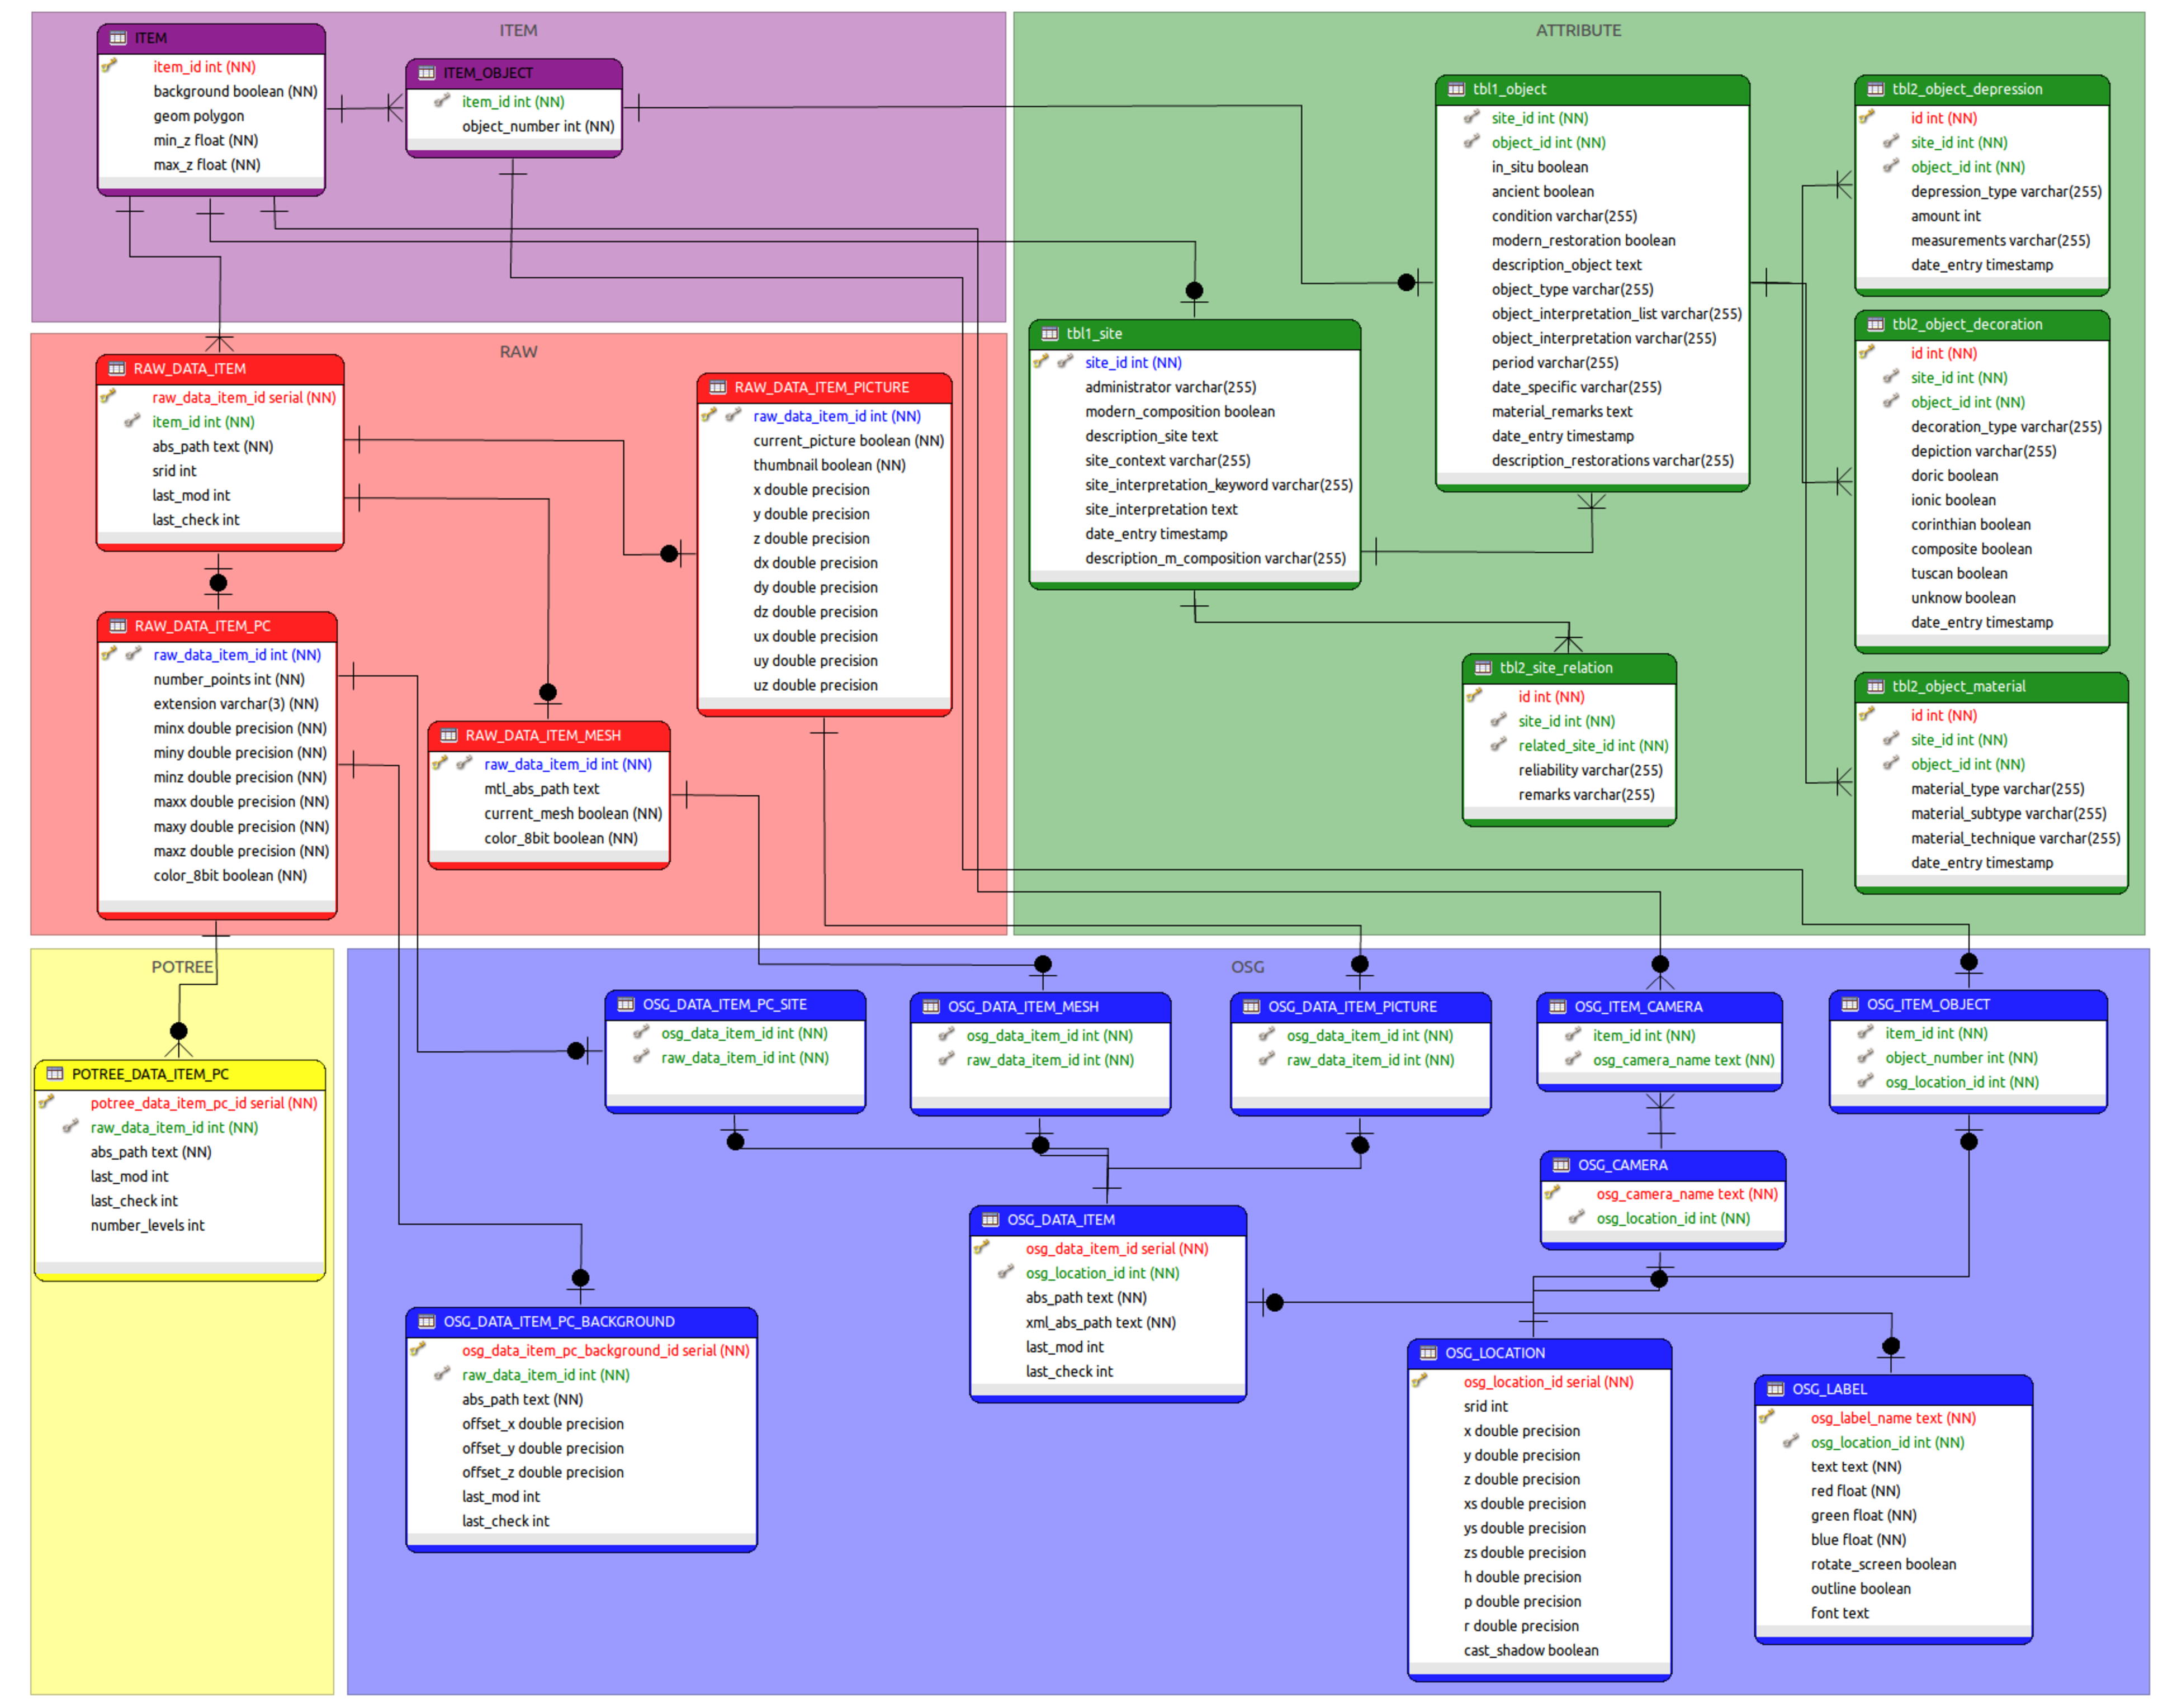
\includegraphics[scale=0.25]{fig/database/ERDB.pdf}
\caption{Entity-Relationship diagram of the \textit{viaappiadb} database with
its five categories.}
\label{fig:db_erdb}
\end{figure}

\subsection{Database logical schema categorization}
In this section describes each category and on each category the tables to store raw
data, converted data, visualization-related data and the footprints (geometries) of
the sites are located.

\subsubsection{ITEM}
Conceptually {\em ITEM} is a category containing an information about an {\em item}.
Item is any entity of interest- background (then the logical field {\em background} is
set to true (1)) or site (0). If the item of interest is an archaeological site (monument)
it contains one or more objects (parts of the site) which is reflected by the field
{\em object\_numer}. 

Figure \ref{fig:db_erdb_item} shows the relationship of the {\em ITEM} category with
the other categories. The {\em ITEM} category is on the top of the categories' hierarchy.

\begin{figure}[H]
\centering
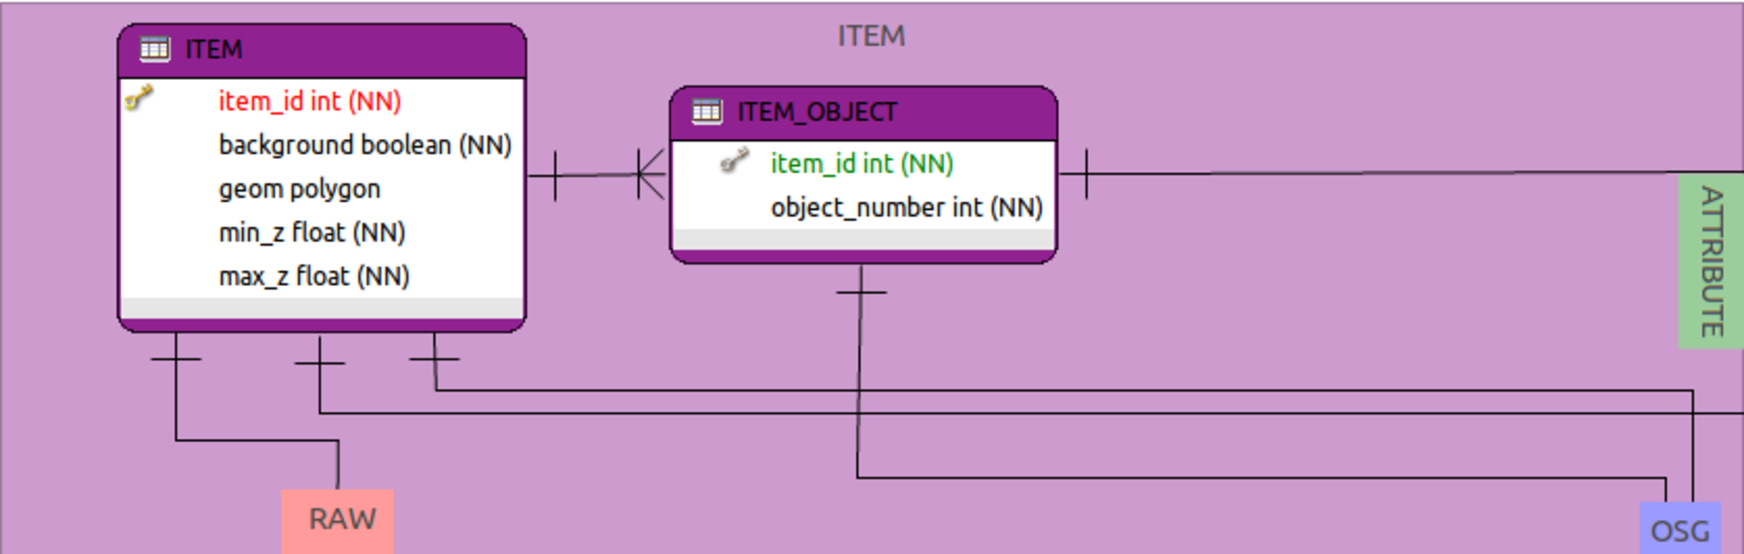
\includegraphics[scale=0.35]{fig/database/ERDB_ITEM_conn.pdf}
\caption{Entity-Relationship diagram of category ITEM and indicated connections
with other categories.}
\label{fig:db_erdb_item}
\end{figure}

\subsubsection{RAW}
The {\em RAW} category contains all the \textit{raw data} gathered for given item.
The most important meta-data is the location in the Data structure (Section~\ref{sec:data_structure}),
stored in the {\em abs\_path} field. These data can be either point clouds (PC),
meshes (MESH) or pictures (PICTURE). Each of these types is represented by a separate
table with the specific for that data type properties. The {\em RAW} category is
related to the derived data categories {\em OSG} and {\em POTREE} as indicated on
Figure~\ref{fig:db_erdb_raw}.

\begin{figure}[H]
\centering
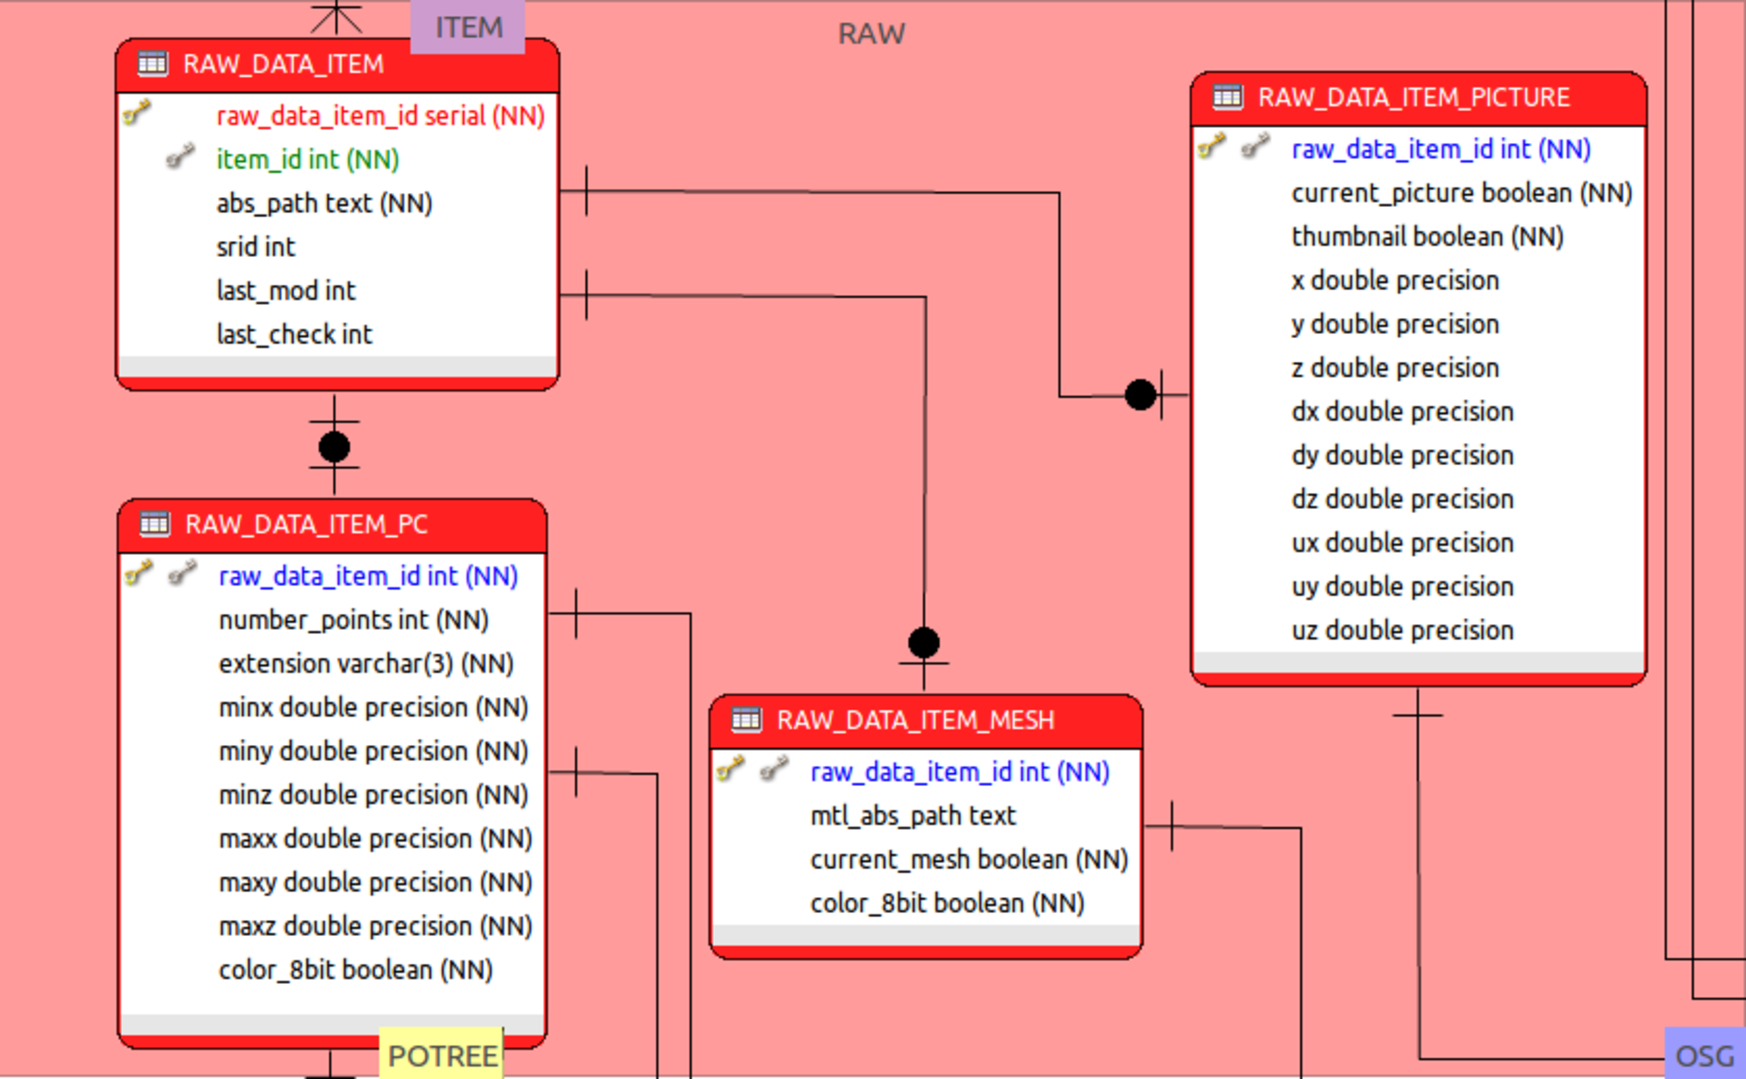
\includegraphics[scale=0.35]{fig/database/ERDB_RAW_conn.pdf}
\caption{Entity-Relationship diagram of category {\em RAW} and indicated connections
with other categories.}
\label{fig:db_erdb_raw}
\end{figure}

\subsubsection{OSG}
The {\em OSG} category represents the OSG \textit{converted data} used for the
desktop based viewer. Figure \ref{fig:db_erdb_osg} it is related to the RAW data
(from where it is derived) and to the ITEM category. The tables in this category
reflect the possible data types: PC, meshes and pictures. Most importantly, this
category contains information needed for the \textit{visualization}, like specifics
of the background and items, the camera, location (bounding box) and label. 

\begin{figure}[H]
\centering
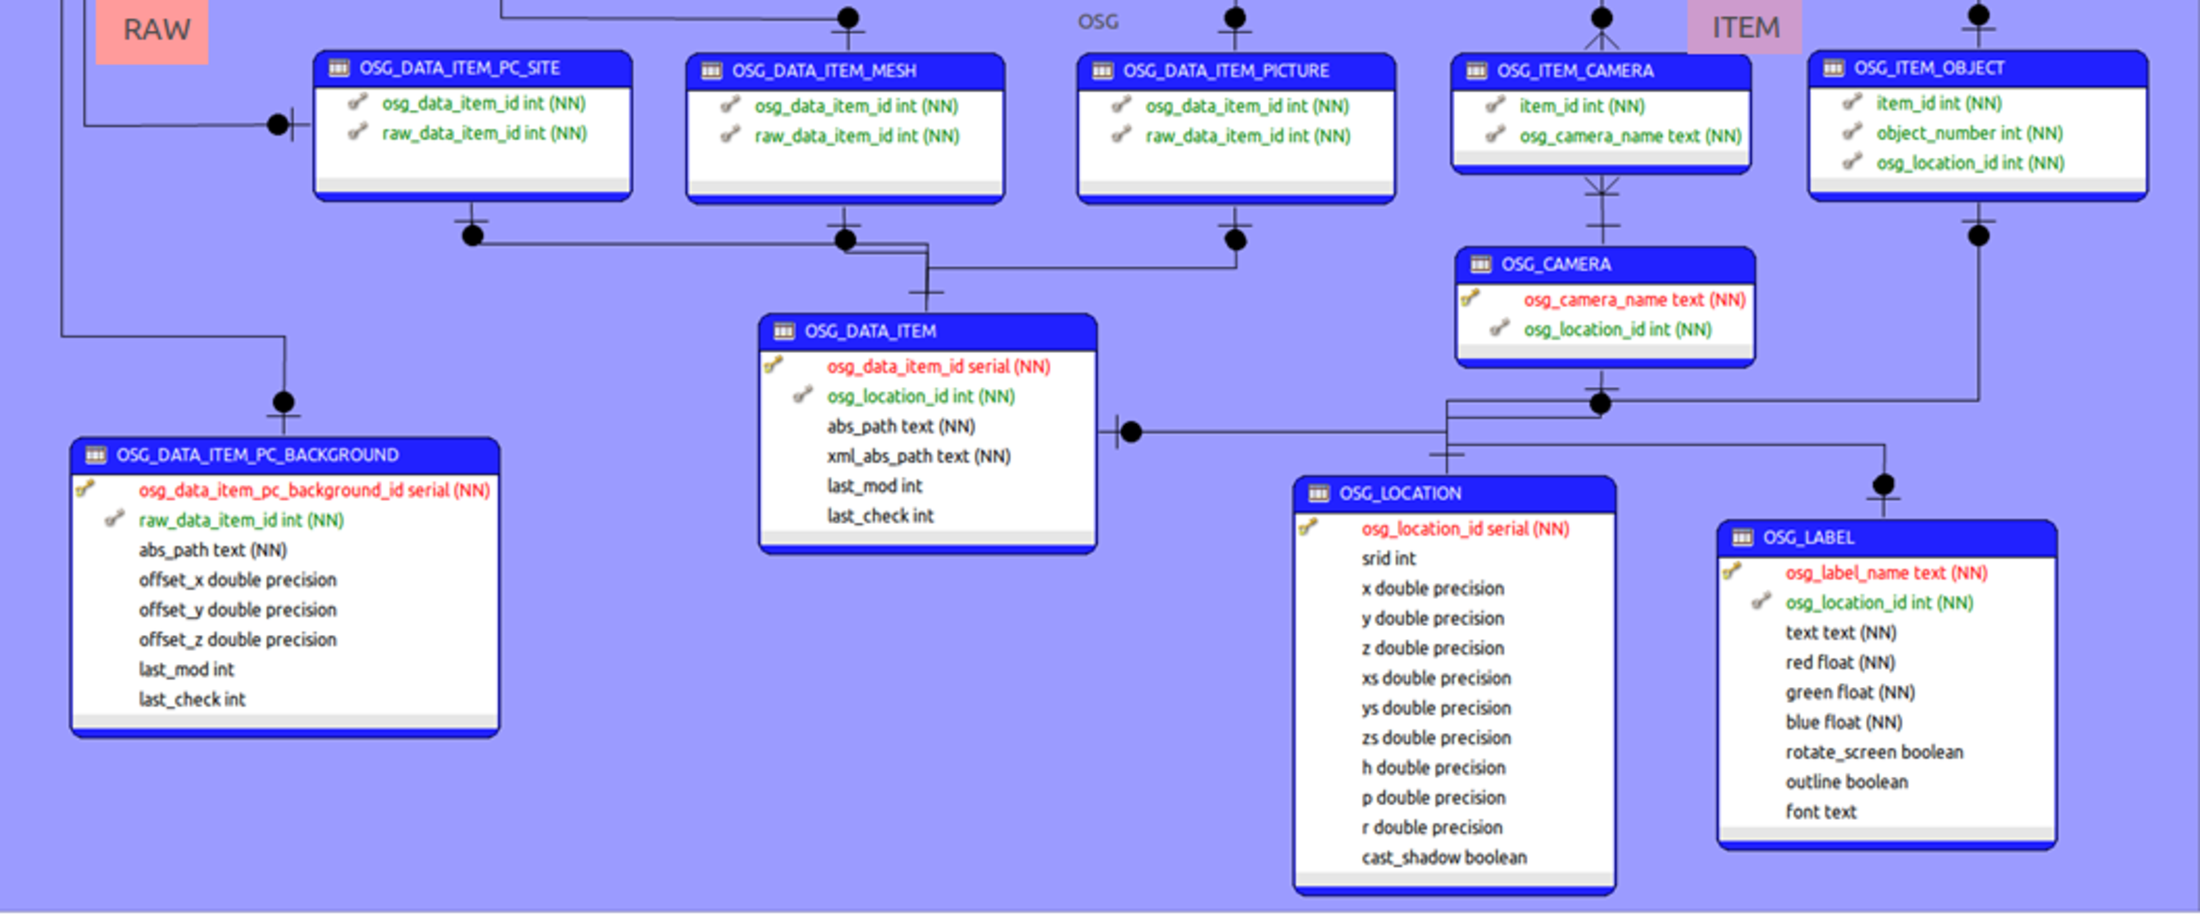
\includegraphics[scale=0.35]{fig/database/ERDB_OSG_conn.pdf}
\caption{Entity-Relationship diagram of category {\em OSG} and indicated connections
with other categories.}
\label{fig:db_erdb_osg}
\end{figure}

\subsubsection{POTREE}
The {\em POTREE} category is illustrated on Figure \ref{fig:db_erdb_potree}. It
is related only to the {\em RAW} category from which it is derived using the Potree
converter and stores only data of the PC type and conversion parameters ({\em number\_levels}).

\begin{figure}[!H]
\centering
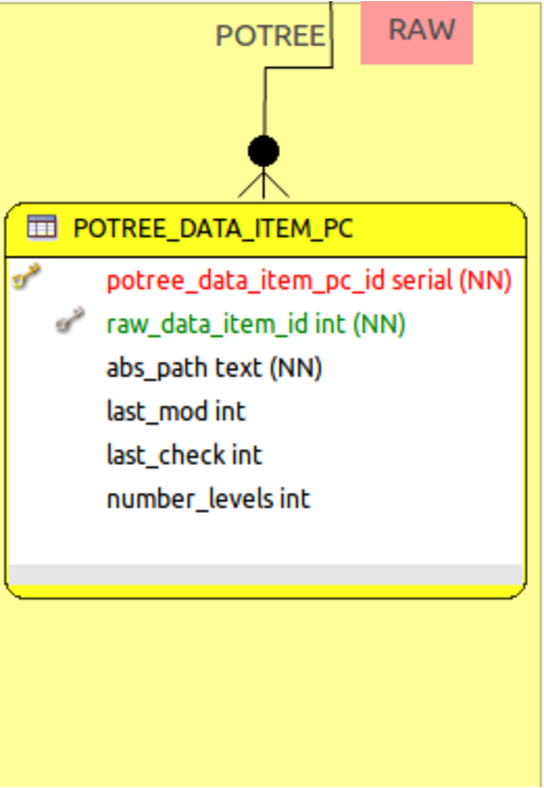
\includegraphics[scale=0.35]{fig/database/ERDB_POTREE_conn.pdf}
\caption{Entity-Relationship diagram of category {\em POTREE} and indicated
connections with other categories.}
\label{fig:db_erdb_potree}
\end{figure}

\subsection{Attribute data}
The attribute part of the DB is represented only by one category, {\em ATTRIBUTE}
(Figure \ref{fig:db_erdb_attribute}). It is connected only to the {\em ITEM} category.
These are the meta-data collected during the field work and are primarily of research
interest to the archaeologists as it contains all domain-related data enabling browsing
and filtering of sub-parts of the data of interest.

\begin{figure}[H]
\centering
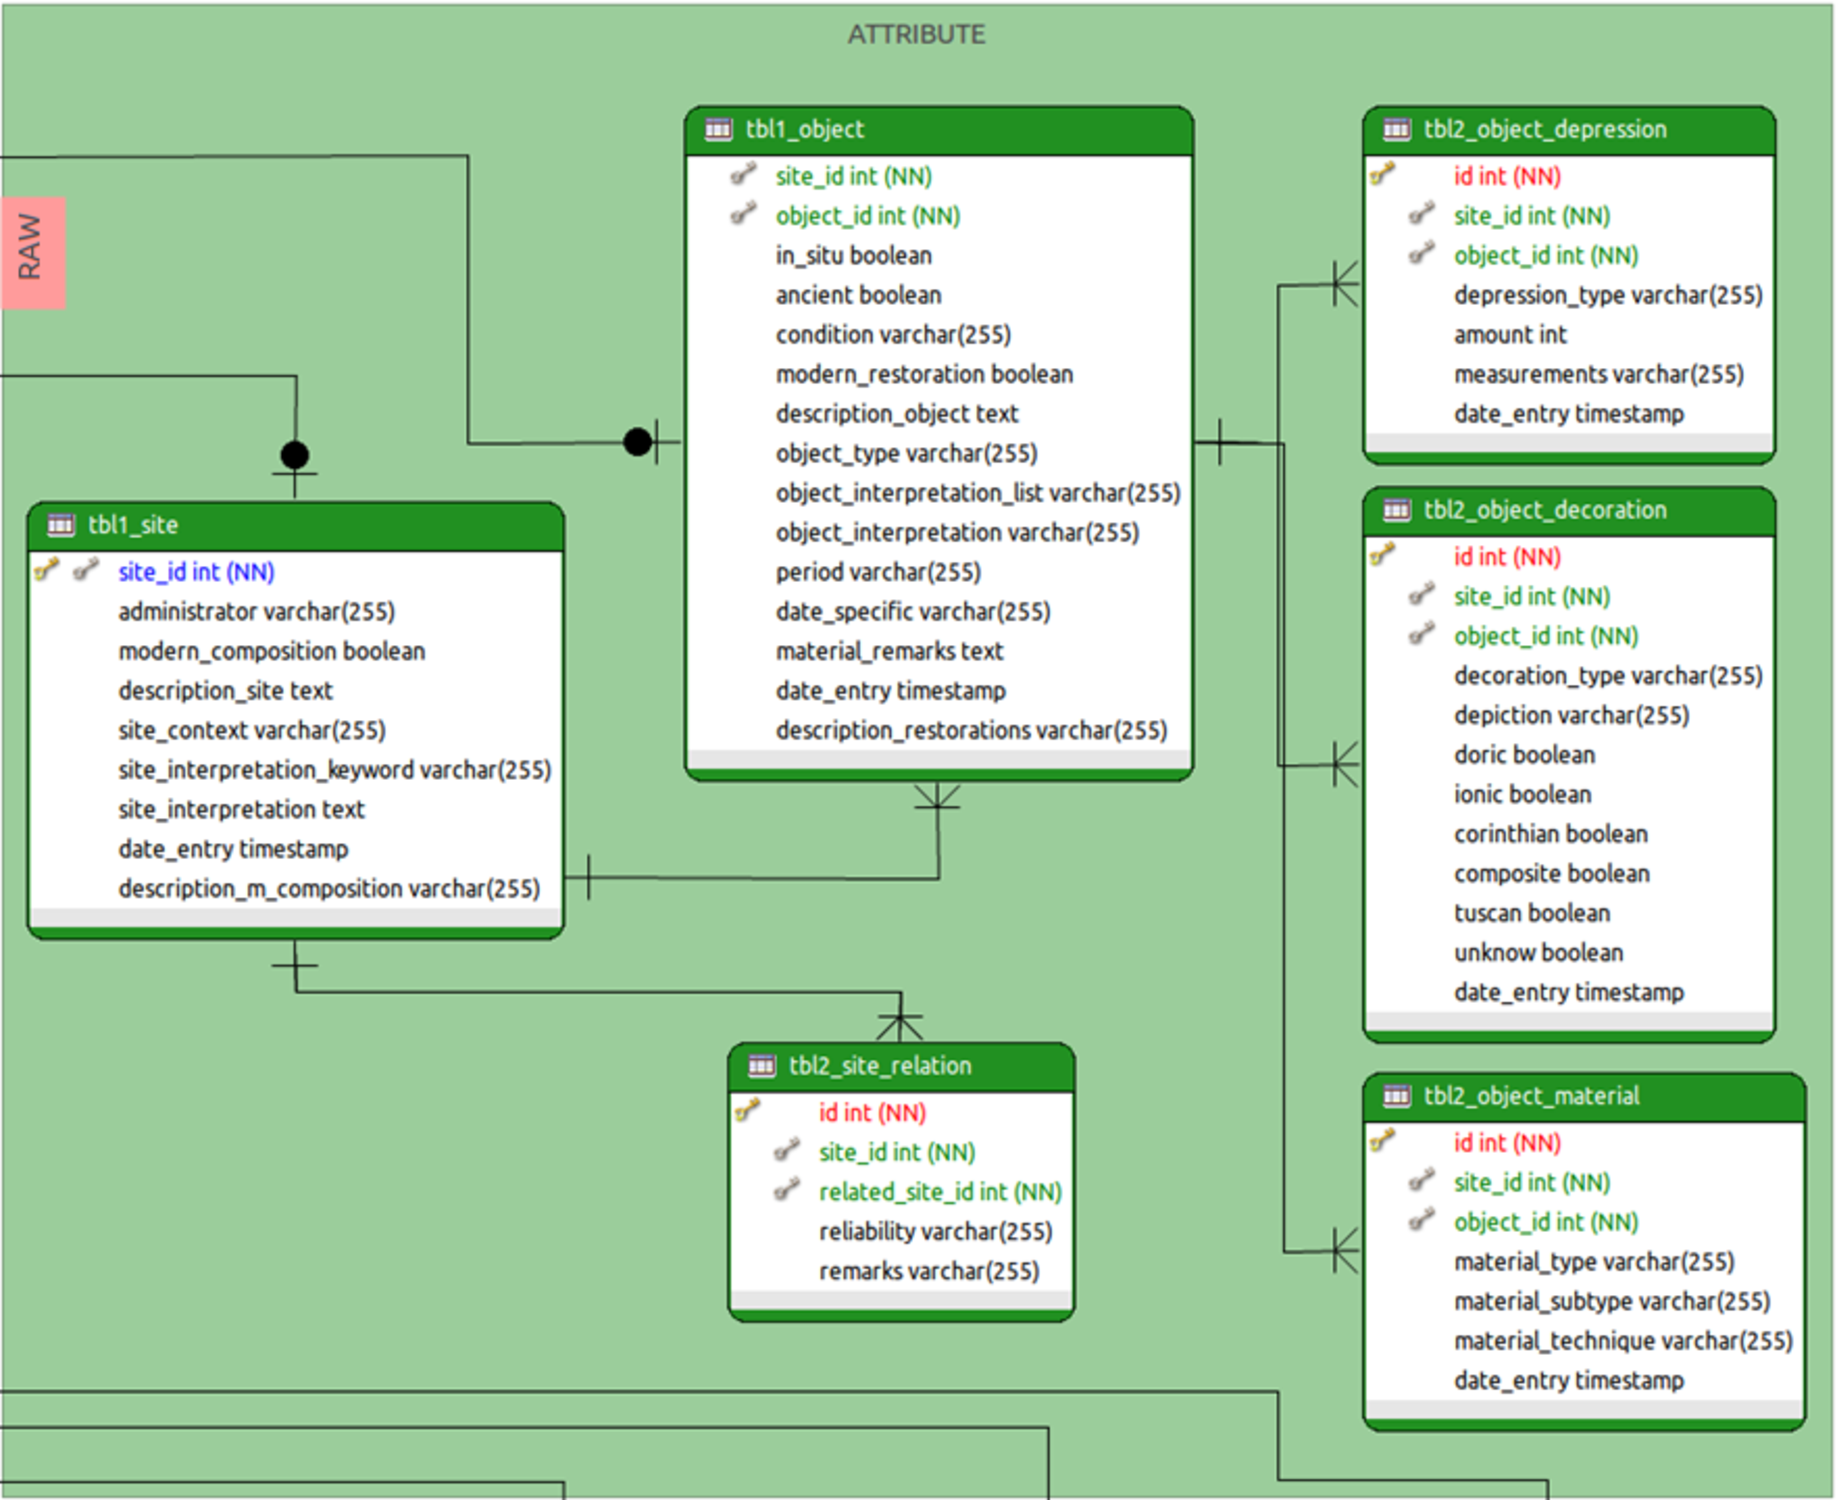
\includegraphics[scale=0.35]{fig/database/ERDB_ATTRIBUTE_conn.pdf}
\caption{Entity-Relationship diagram of category {\em ATTRIBUTE} and indicated
connections with other categories.}
\label{fig:db_erdb_attribute}
\end{figure}

The \textit{viaappiadb} database is running in the Via Appia Linux server. See
Section~\ref{sec:software} on how to get an account in the database.



\section{Software}
\label{sec:software}
As described in section \ref{sec:sys_arch} the 4D GIS system has a two tier
architecture, the server and the clients. 

\subsection{Server software}
The \textit{viaappiadb} database running in the Via Appia Linux server is a
PostgreSQL 9.2.8 with PostGIS 2.1.2 and GDAL 1.10.0.

Specific point cloud libraries are also used for the management and processing
of point cloud data, concretely LASzip, libLAS and LAStools. In LAStools and
libLAS many of their applications share the same name and in these cases the
usage of the LAStools ones is preferred. In order to guarantee this we need to
set the \textit{PATH} environment variable accordingly, i.e. by setting the
LAStools bin folder prior to the libLAS one.

As described in section \ref{sec:data_structure} the data stored in the server
needs to be converted to the specific formats required by the two supported
visualizations, i.e. the web viewer based on Potree and the Windows desktop
viewer/editor based on Open Scene Graph. To perform these conversions we use
the \textit{PotreeConverter} (https://github.com/potree/PotreeConverter) and
the \textit{OSGConverter}
(https://github.com/NLeSC/Via-Appia/tree/master/converter) which requires the
Open Scene Graph (we currently use 3.2.1). Both converters use Boost (our
installed version is 1.55).

An NGINX web server is also used to serve files (static content) to the
web-based visualization. 

\subsection{Client software}
The web visualization viewer only requires the installation of a modern web
browser in the client laptop/desktop (we have used Chrome/Chromium).

For the desktop-based visualization we use a tool based on OpenSceneGraph (OSG)
so the point cloud data and also the pictures and meshes have to be converted
to OSG format. This conversion also happens in the Via Appia server and it is
executed by a

For the usage of the OSG desktop viewer some additional libraries have to be
installed

{\em pasted form old documentaiton- to be edited!}
 
In order to use the new 4D GIS system the end-user only needs to do:
\begin{itemize} \item (a.) Obtain an account in the Via Appia Linux server and
in the \textit{viaappiadb} database and generate a SSH key pair (see
Subsections \ref{sec:accounts} and \ref{sec:sshkeys}).  \item (b.) Download,
install and configure the \textit{launcher} tool in his Windows laptop or
desktop (see Subsection \ref{sec:install}).  The \textit{launcher} tool also
contains the 4D viewer. It is also recommend to install two tools for the
communication between the Linux server and the Windows computers: PuTTY and
WinSCP (see Subsubsections \ref{sec:putty} and \ref{sec:winscp}).
\end{itemize}

The database is a PostgreSQL 9.2.8 (version correct?) instance running with
PostGIS 2.1.2.

We also need the python binding of GDAL and LiblAS.


\end{document}

